\documentclass{beamer}
% Nächstes Auskommentieren um jedes \pause zu 'deaktivieren'!
%\documentclass[handout]{beamer}

\usepackage{talk_BeamerColor}

\usepackage[pantoneblack7,english]{talk_wwustyle_LA}

\usepackage[ngerman]{babel}
\usepackage[utf8]{inputenc}
\usepackage[T1]{fontenc}
\usepackage{lmodern}
% --- Paket um Grafiken im Dokument einbetten zu koennen
\usepackage{graphicx}
\usepackage{caption}
\usepackage{subfigure}
\usepackage{wrapfig}
\usepackage{tikz}

% --- Pakete fuer mathematischen Textsatz
\usepackage{amsmath}
\usepackage{amssymb}
\usepackage{empheq}
\usepackage{dsfont}		
\usepackage{amstext}
\usepackage{amsfonts}
\usepackage{amsthm}
\usepackage{wasysym}

% --- Paket erweitert deutlich die Verwendung von Farben aus dem Paket 'graphicx'
\usepackage{color}

% --- Paket um Quellcode sauber zu formatieren
\usepackage{listings}

% --- Darstellung von Pseudocode und mehr (algorithmicx packages)
\usepackage{algorithm}
\usepackage{algpseudocode}

%% Physikalisches
\usepackage{nicefrac}
\usepackage{units}
\usepackage{siunitx}
\sisetup{
  inter-unit-product 	=	$\cdot$,
  fraction-function   	= 	\nicefrac,
  load-configurations 	= 	abbreviations,
  per-mode            	= 	fraction,
  separate-uncertainty	=	true,
  output-decimal-marker	=	{.}
  }   
\usepackage{isotope}

%% Aufgabenverwaltung
\usepackage[textwidth=2cm,% Breite der Todo-Eintr�ge
            textsize=footnotesize,% Schriftgr��e der Eintr�ge
            english,% deutsche Beschriftungen
            shadow,% Schlagschatten f�r Boxen (weils so h�bsch ist)
            colorinlistoftodos]{todonotes}% farbige Markierungen f�r unterschiedliche Aufgabentypen
\newcommand{\detail}[1]{\todo[color=Green,inline]{detail: #1}~}% Details k�nnten hinzugef�gt werden
\newcommand{\litcheck}[1]{\todo[color=LightSteelBlue,inline]{refcheck: #1}~}% muss noch einmal �berpr�ft werden
\newcommand{\src}[1][]{\todo[color=Tomato,inline]{reference! #1}~}% Quelle fehlt

% % Zusätzliches:
\usepackage{braket}
\usepackage{epstopdf}
\usepackage{pgfpages}
\usepackage{csquotes}

\newlength{\halftextwidth}
\setlength{\halftextwidth}{\textwidth}
\divide\halftextwidth by 2

% --- Einstellungen

\author{NiMoNa (Zwischenpräsentation) SoSe 2016}
\title{Konnektivität im Gehirn}
%\institutelogo{Logo on title frame}
%\institutelogosmall{Logo on other frames}
\subtitle{Lutz Althüser, Tobias Frohoff-Hülsmann, Victor Kärcher,\\ Lukas Splitthoff, Timo Wiedemann\\ Unterstützt durch: Christian Himpe}
\date[08.06.2016]{08. Juni, 2016}

% --- Beginn des Dokuments

\begin{document}

\begin{frame}[plain]
	  \maketitle
\end{frame}

\begin{frame}{Überblick}
	\tikz[remember picture,overlay]
		  \node at ([xshift=-2.8cm,yshift=-5cm]current page.north east)
		  {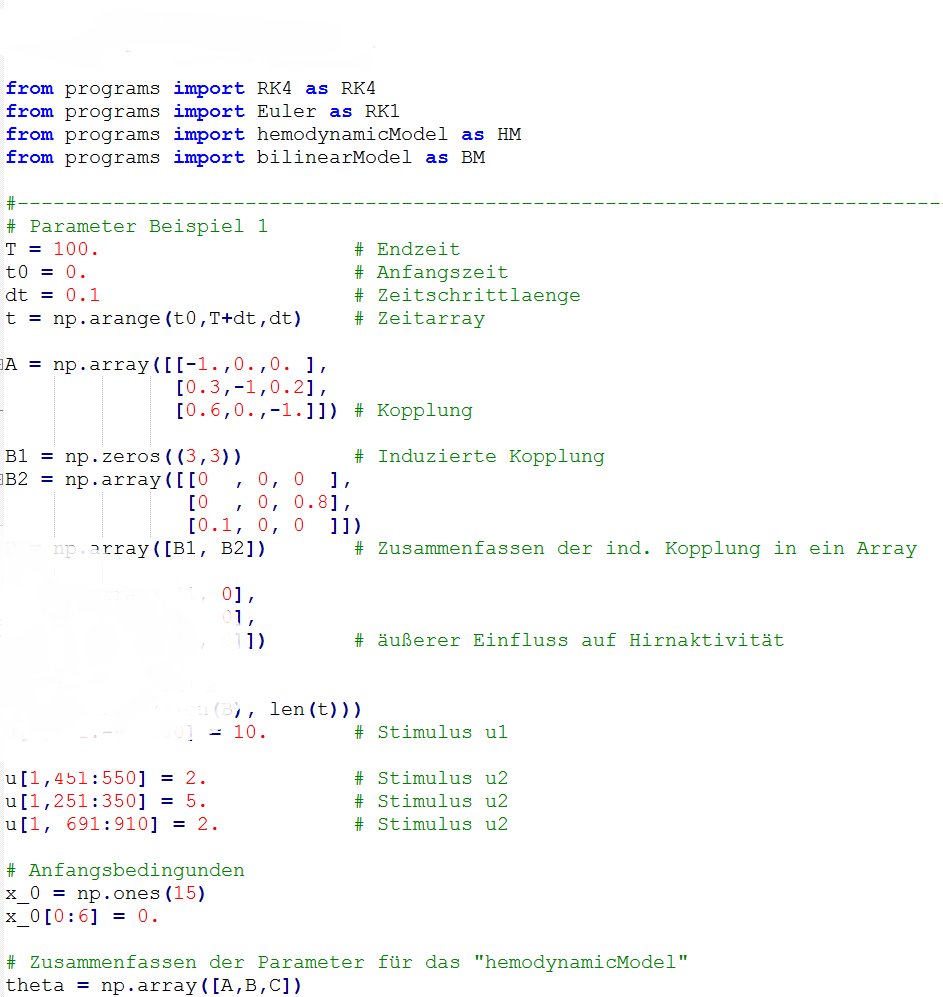
\includegraphics[height=7cm,angle=-7.5,keepaspectratio]{res/toc_2.png}};
	  \tableofcontents
\end{frame}

\section{Motivation und Ziel}
	\begin{frame}{Einleitung in DCM - \underline{D}ynamic \underline{C}ausal \underline{M}odelling}
		\begin{columns}
		\column[t]{6cm}
		\begin{figure}
			\centering
			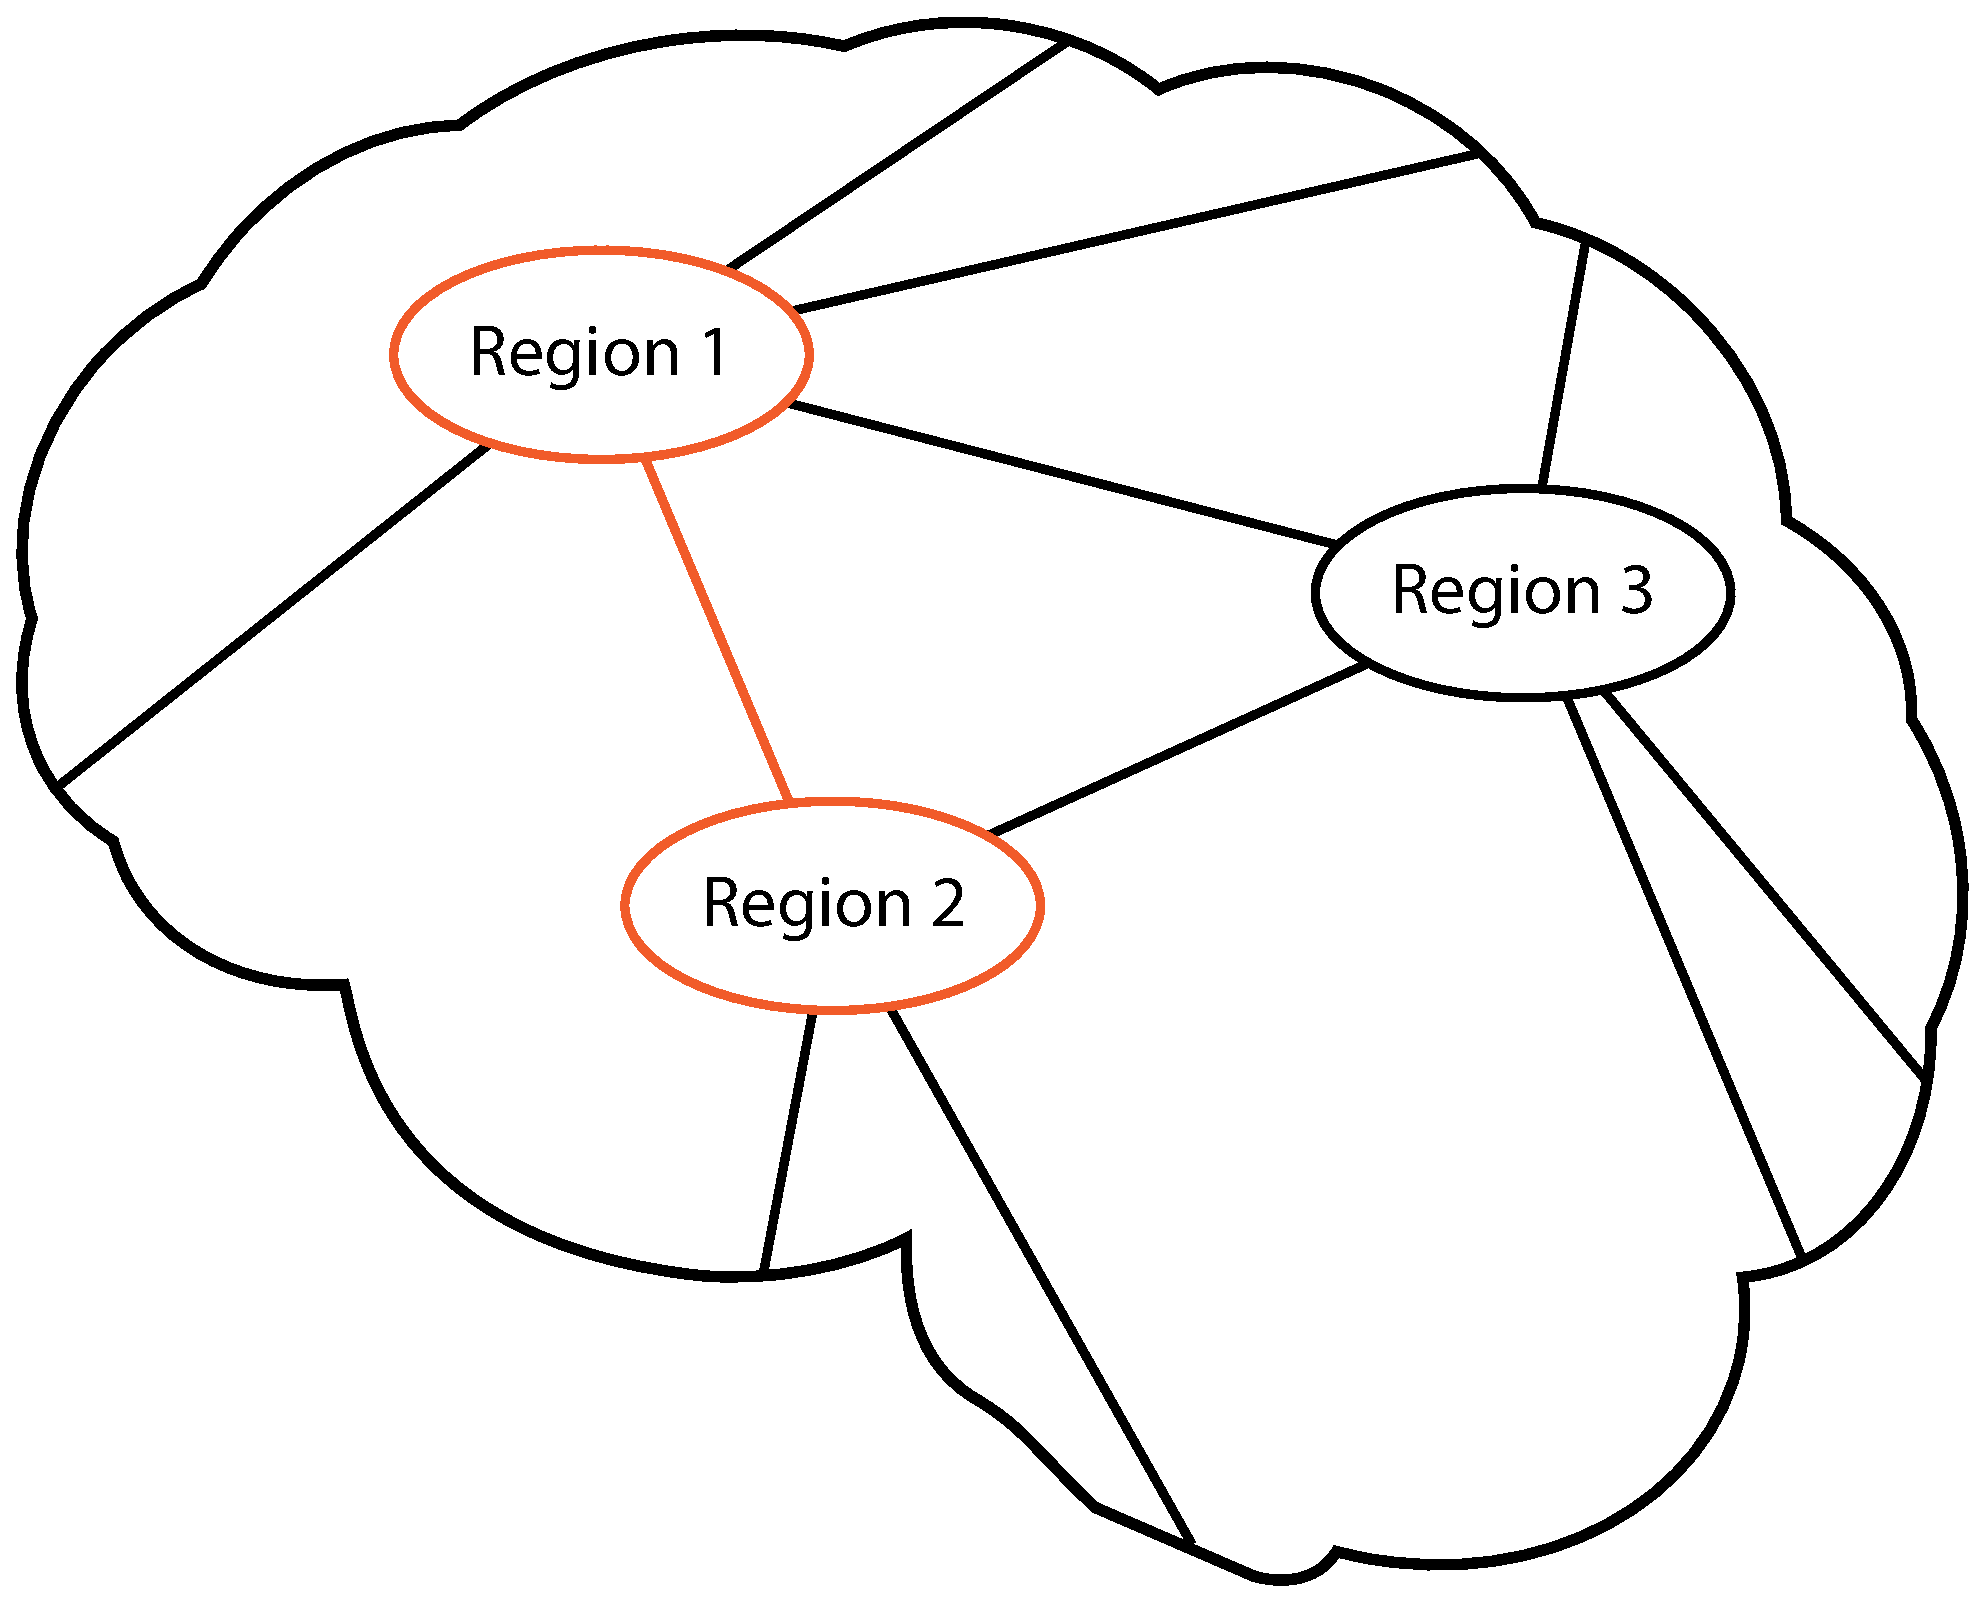
\includegraphics[width=0.85\linewidth]{res/brain_01.eps}
			\\ {\small Interaktion zwischen}\\ {\small verschiedenen Hirnregionen}
			\label{fig:brain_01}
		\end{figure}
		\column[t]{6cm}
		\begin{block}{\centering Konnektivität im Gehirn}
			\centering
			Über die mathematische Modellierung von Interaktionen zwischen mehreren Regionen des Gehirns.
		\end{block}
		\vspace{0.5cm}
		\begin{exampleblock}{\centering Ziel}
			 \centering
			 Das Aufstellen eines einfachen und realistischen neuronalen Modells aller betrachteten interagierenden Gehirnregionen.
		\end{exampleblock}
		\end{columns}
		\vskip0pt plus 1filll
	\end{frame}
	
	%\begin{frame}{Einleitung in DCM - \underline{D}ynamic \underline{C}ausal \underline{M}odel}
	%	\begin{columns}
	%		\column[t]{6cm}
	%		\centering [Hier ein nettes Bild]
	%		\column[t]{6cm}
	%		\begin{exampleblock}{\centering Ziel}
	%			 \centering
	%			 Das Aufstellen eines einfachen und realistischen neuronalen Modells aller interagierenden Gehirnregionen.
	%		\end{exampleblock}
	%	\end{columns}
	%	\vfill
	%	\begin{itemize}
	%		\item Rückschlüsse auf die Verschaltung von Hirnregionen
	%		\item Einfluss der Veränderungen in der neuronalen Aktivität
	%	\end{itemize}
	%	\vfill
	%	\begin{center}
	%		Datengrundlage des DCM sind funktionelle Magnetresonanztomographien.
	%	\end{center}
	%\end{frame}
	
\section{DCM Modelle}
\subsection{Lineares Modell}
	\begin{frame}{Lineares Modell}
		\begin{columns}
			\column[t]{4cm}
			\begin{figure}
				\centering
				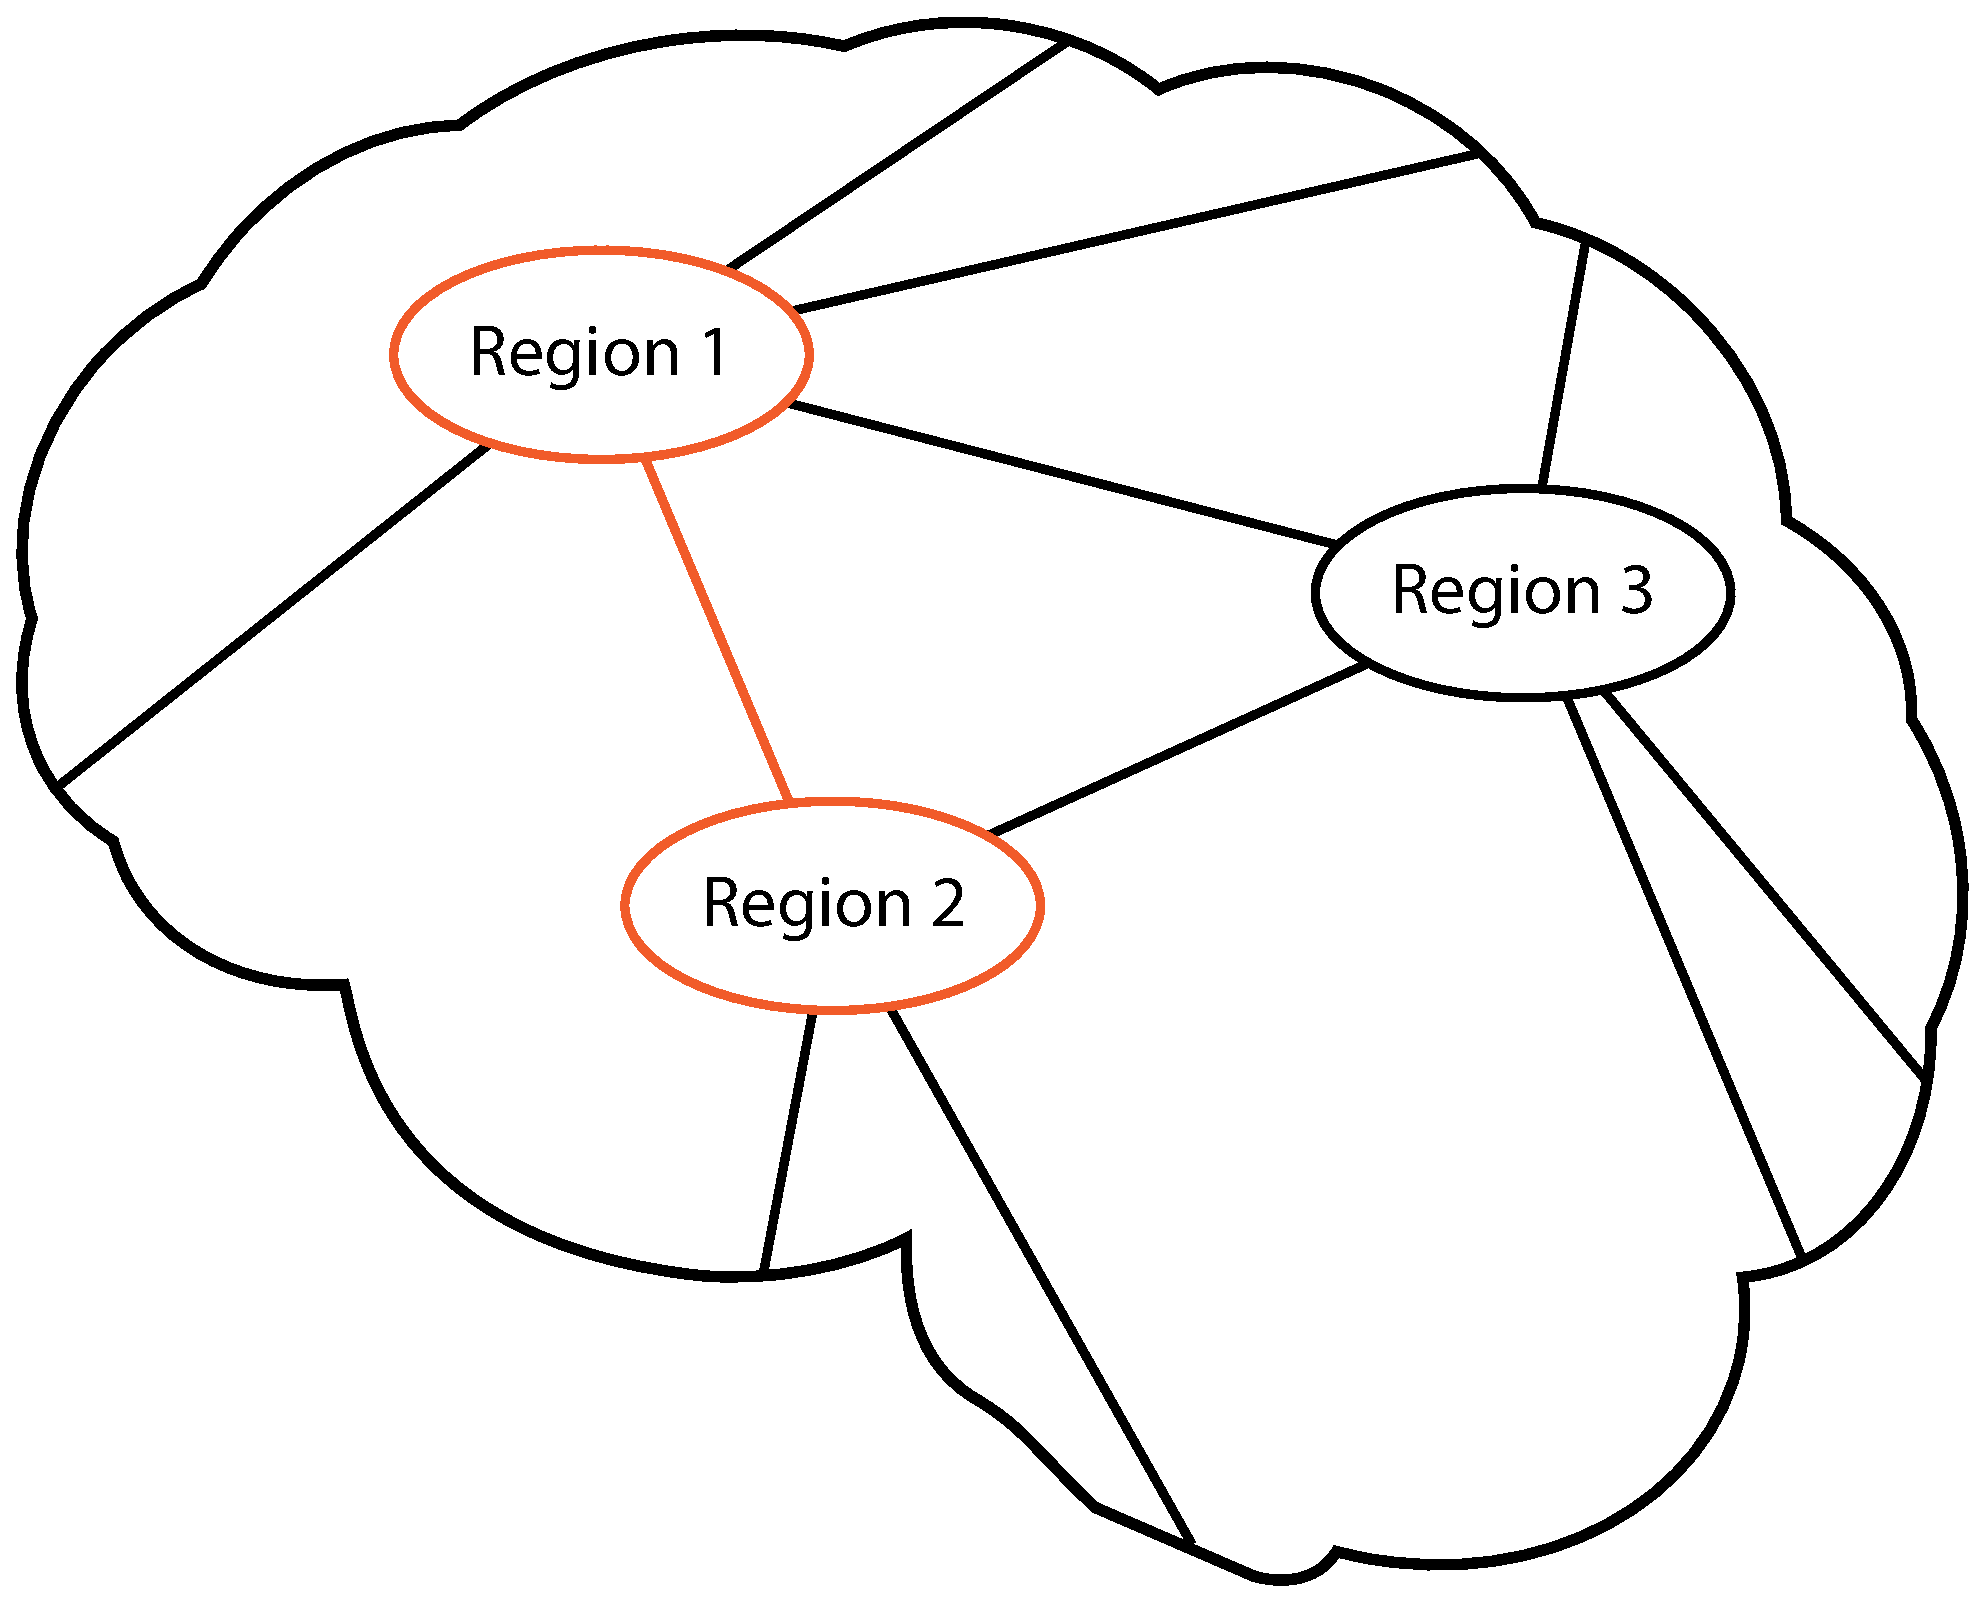
\includegraphics[width=0.85\linewidth]{res/brain_01.eps}
				\\ {\small Vernetzung von} \\{\small Hirnregionen}
				\label{fig:brain_02}
			\end{figure}
			\column[t]{8cm}
			\begin{center}
				Inputs $u$ $\rightarrow$ Outputs $z$ pro Hirnregion\\ 
				\vspace{0.25cm}
				\scalebox{.5}{
					\begin{minipage}{\textwidth}
					\begin{block}{Inputs}
						\begin{itemize}
						\item direkten Input: Stimulation $u$ der Hirnregion
						\item ...
						\end{itemize}
					\end{block}
					\end{minipage}
					\hfill
					\begin{minipage}{\textwidth}
					\begin{block}{Outputs}
						\begin{itemize}
						\item neuronale Aktivität in der Hirnregion
						\item ...
						\end{itemize}
					\end{block}
					\end{minipage}
				}\\
				\vspace{0.5cm}
				$\dot{z}=A+Cu$ 
			\end{center}
		\end{columns}	
		\vspace{0.5cm}
		\begin{small}
		Matrix $A$: Konnektivitätsmatrix - Verschaltung der Hirnregionen \\
		Matrix $C$: Einfluss der Inputs auf die neuronale Aktivität einer Hirnregion
	\end{small}		 
	\end{frame}
	
\subsection{Bilineares Modell}
%	\begin{frame}{Bilineares Modell}
%		\begin{figure}
%			\centering
%			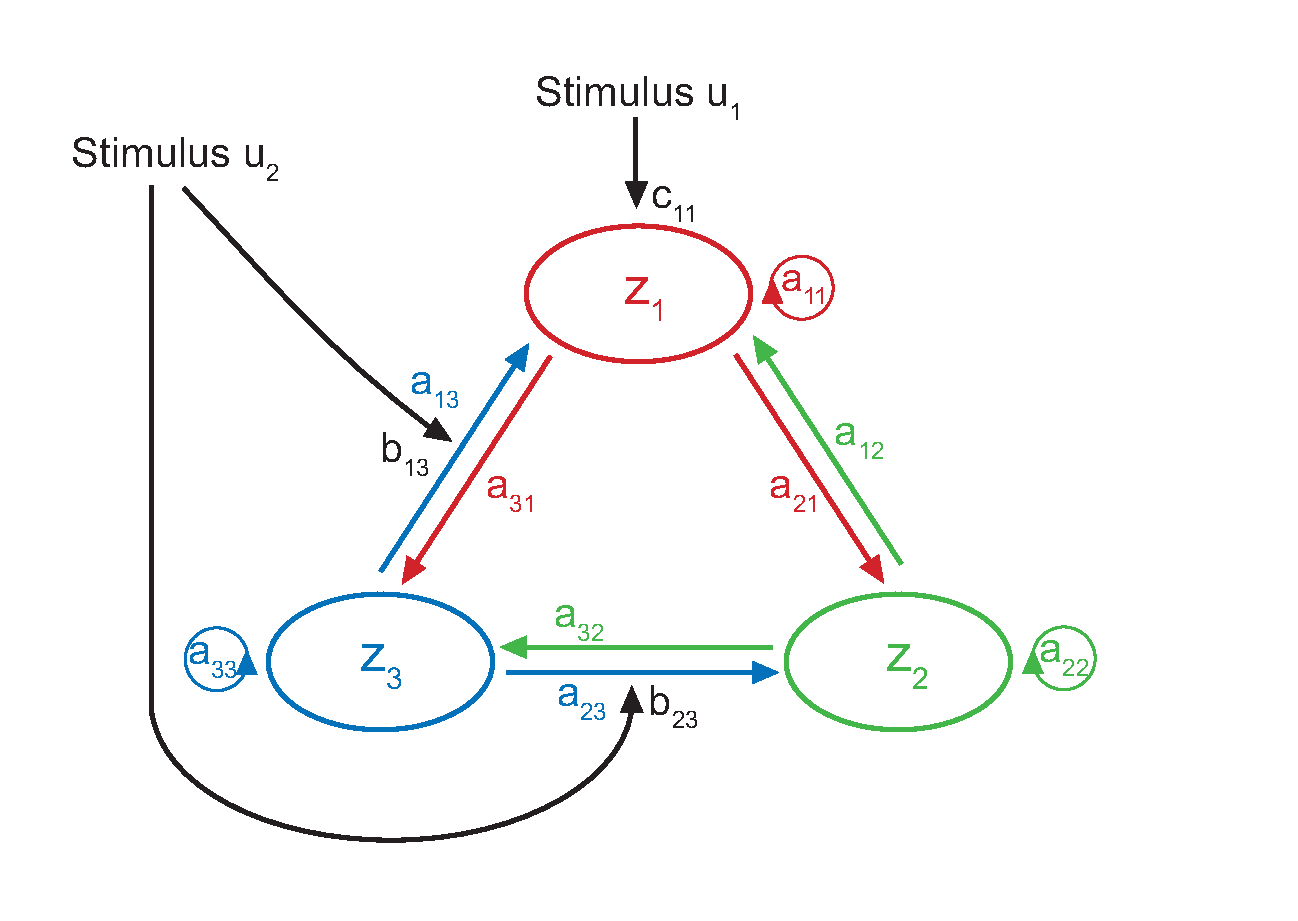
\includegraphics[width=0.60\linewidth]{res/bilinearesModell_neu.eps}
%			\label{fig: bilinearesModel}
%		\end{figure}
%		\begin{columns}[c]
%			\column[t]{7cm}
%			\centering
%			\scalebox{.6}{
%				\begin{minipage}{\textwidth}
%					\begin{block}{Modell}
%						\begin{itemize}
%							\item n verschiedene Gehirnregionen mit der Zustandsvariablen $ z_i $ mit $ i=1,...,n $
%							\item Aktivität durch vorgegebene Eingangssignale bestimmt
%						\end{itemize}
%					\end{block}
%				\end{minipage}
%			}				
%			\column[t]{7cm}				
%				\scalebox{.6}{
%					\begin{minipage}{\textwidth}
%						\begin{block}{Input $ u_1 $, $ u_2 $}					%Ggf. diesen Block inhaltlich änder, da Dopplung
%							\begin{itemize}
%								\item direkten Input $ u_1 $: Veränderung des neuronalen Zustands
%								\item latenten Input $ u_2 $: Veränderung der Vernetzung
%							\end{itemize}
%						\end{block}
%					\end{minipage}
%			}	
%		\end{columns}	
%	\end{frame}
	
	\begin{frame}{Bilineares Modell}
		\begin{columns}
			\column[t]{5cm}
				\begin{figure}
					\centering
					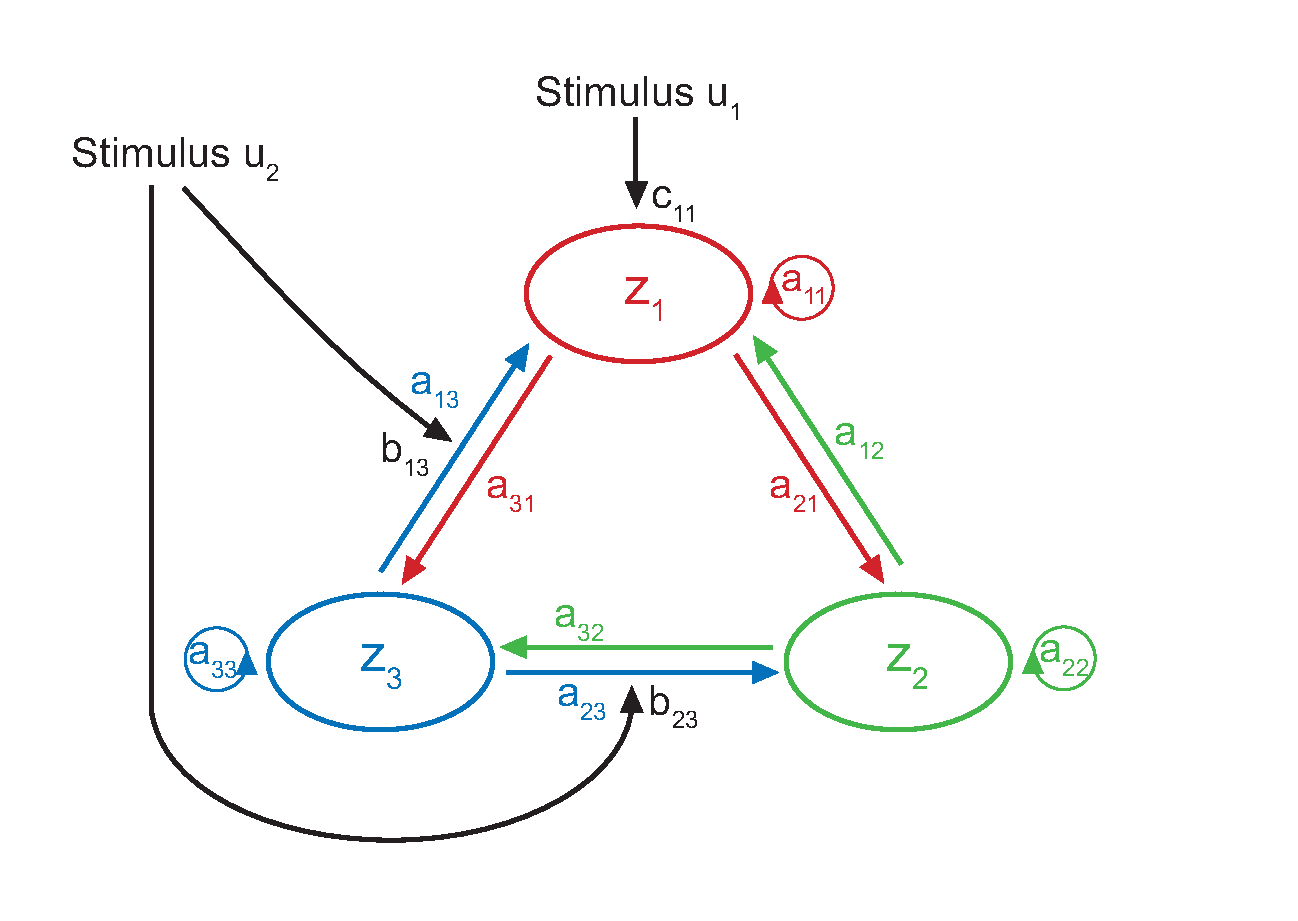
\includegraphics[width=0.95\linewidth]{res/bilinearesModell_neu.eps}
				\end{figure}
				\centering
				\scalebox{.95}{
					\begin{minipage}{\textwidth}
						\begin{block}{Mathematische Beschreibung}
							\begin{itemize}
								\item Modellierung basierend auf Taylorentwicklung
								\item Dynamik und Konnektivität durch drei Parameter beschrieben
							\end{itemize}
						\end{block}
					\end{minipage}
				}
			\column[t]{9cm}
			Taylorentwicklung
			\scalebox{.7}{
				\begin{minipage}{\textwidth}					
					$
					f(z,u) \approx f(0,0)+\frac{\partial f}{\partial z}z+\frac{ \partial f}{\partial u} u + \frac{\partial^2 f}{\partial z \partial u}zu
					$
				\end{minipage}
			}
			\pause %Pausennummer funktioniert wie?
			\\ \vspace{10pt}
			Bsp: Aktivität der Region 1
				\scalebox{.7}{
					\begin{minipage}{\textwidth}					
					$
					\dot{z}_1 =a_{11}z_1+a_{12}z_2+a_{13}z_3+u_2b_{13}^{(2)}+c_{11}u_1
					$
					\end{minipage}
				}
				\pause %Pausennummer funktioniert wie?
				\scalebox{.98}{
				\begin{minipage}{\textwidth}					
					\vspace{14pt}
					\hspace{5pt}
					$
					\dot{z} =(A+\sum_{i}u_iB^{(i)})z+Cu
					$
				\end{minipage}	
			}
			\scalebox{.7}{
				\begin{minipage}{\textwidth}		
					\vspace{16pt}
					$ A=
					\begin{pmatrix}
					a_{11} & a_{12} & a_{13}\\
					a_{21} & a_{22} & a_{23}\\
					a_{31} & a_{32} & a_{33}
					\end{pmatrix}
					$
					\hspace{5pt} 
					$ B=
					\begin{pmatrix}
					0	& 0 & b_{13}\\
					0 	& 0 & b_{23}\\
					0	& 0 & 0
					\end{pmatrix}
					$
					\\
					\\
					\\					
					$ C=
					\begin{pmatrix}
					c_{11}	& 0\\
					0 	& 0 \\
					0	& 0  
					\end{pmatrix}
					$										
				\end{minipage}
			}				
		\end{columns}
	\end{frame}
	
	\begin{frame}{Bilineares Modell}
		\begin{columns}
			\column[t]{7cm}
			\begin{figure}
				\centering
				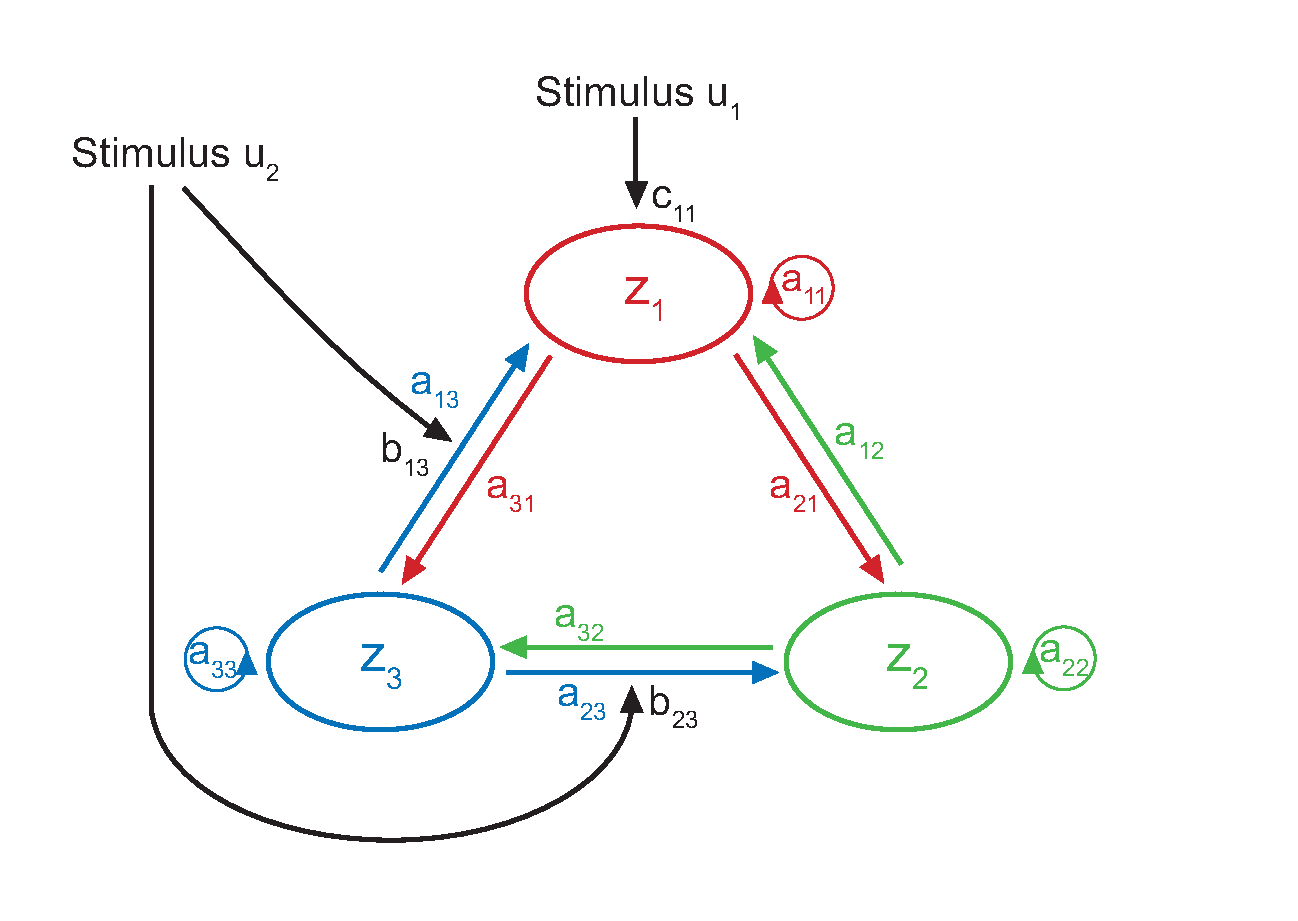
\includegraphics[width=0.65\linewidth]{res/bilinearesModell_neu.eps}
			\end{figure}
			\centering
			\scalebox{.6}{
				\begin{minipage}{\textwidth}
					\begin{block}{Parameter A, B, C}
						\begin{itemize}
							\item A: feste Verknüpfung der Hirnregionen
							\item B: Einfluss des Inputs auf Konnektivität
							\item C: Einfluss des Inputs auf neuronale Aktivität der Hirnregionen
						\end{itemize}
					\end{block}
				\end{minipage}
			}
			\column[t]{7cm}
			Taylorentwicklung
			\scalebox{.7}{
				\begin{minipage}{\textwidth}					
					$
					f(z,u) \approx f(0,0)+\frac{\partial f}{\partial z}z+\frac{ \partial f}{\partial u} u + \frac{\partial^2 f}{\partial z \partial u}zu
					$
				\end{minipage}
			}
			\\ \vspace{10pt}
			Bsp: Aktivität der Region 1
			\scalebox{.7}{
				\begin{minipage}{\textwidth}					
					$
					\dot{z}_1 =a_{11}z_1+a_{12}z_2+a_{13}z_3+u_2b_{13}^{(2)}+c_{11}u_1
					$
				\end{minipage}
			}
			\scalebox{.98}{
				\begin{minipage}{\textwidth}					
					\vspace{14pt}
					\hspace{5pt}
					$
					\dot{z} =(A+\sum_{i}u_iB^{(i)})z+Cu
					$
				\end{minipage}	
			}
			\scalebox{.7}{
				\begin{minipage}{\textwidth}		
					\vspace{16pt}
					$ A=
					\begin{pmatrix}
					a_{11} & a_{12} & a_{13}\\
					a_{21} & a_{22} & a_{23}\\
					a_{31} & a_{32} & a_{33}
					\end{pmatrix}
					$
					\hspace{5pt} 
					$ B=
					\begin{pmatrix}
					0	& 0 & b_{13}\\
					0 	& 0 & b_{23}\\
					0	& 0 & 0
					\end{pmatrix}
					$
					\\
					\\
					\\					
					$ C=
					\begin{pmatrix}
					c_{11}	& 0\\
					0 	& 0 \\
					0	& 0  
					\end{pmatrix}
					$										
				\end{minipage}
			}				
		\end{columns}
	\end{frame}	
	
\subsection{Hämodynamisches Modell}
\begin{frame}{Vergleichbarkeit}
Bilineare Modell $\Rightarrow$ Gehirnaktivitäten $z_i(t)$\\~\\
%\begin{figure}
	%{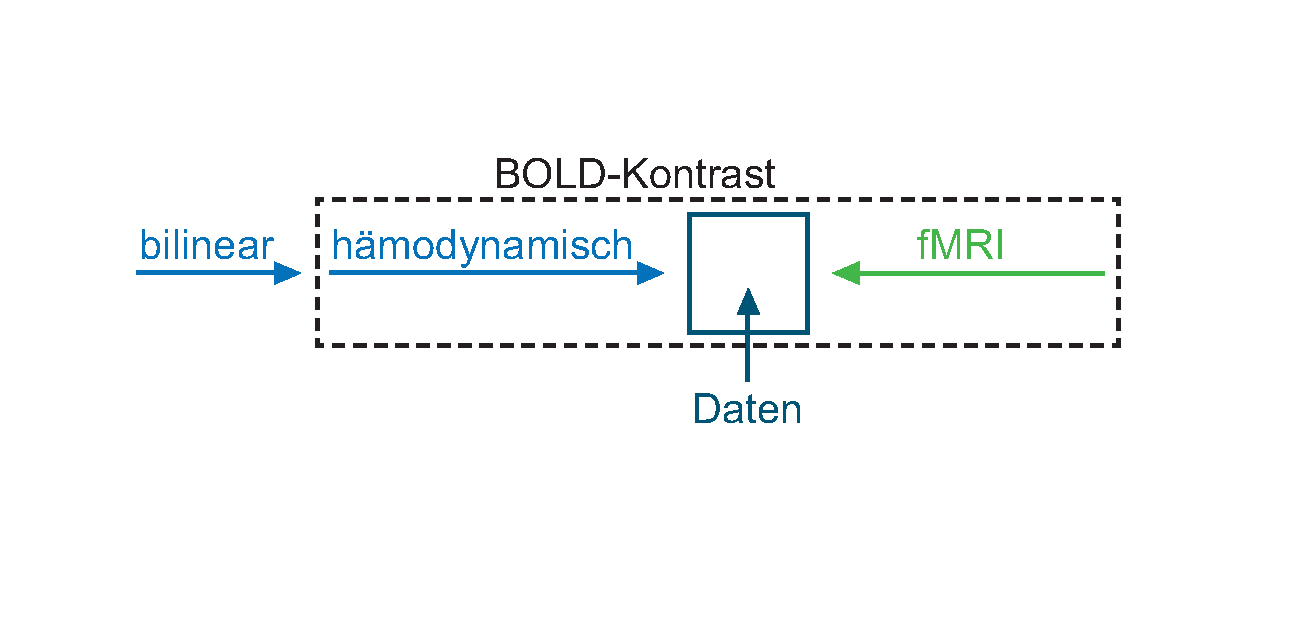
\includegraphics[width=0.8\linewidth]{res/Modelluebersicht_klein.eps}}
%\end{figure}
%\pause
Experiment (funktionelle MRT)$\Rightarrow$ BOLD-Signal/Kontrast $y_i(t)$\\
\hspace{3cm} $\approx$ Sauerstoffgehalt der roten Blutkörperchen 
\begin{figure}
{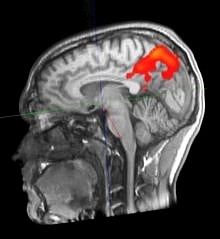
\includegraphics[width=0.3 \textwidth]{res/bold_signal.jpg}}
\end{figure}
\end{frame}

\begin{frame}{Hämodynamisches Modell}
4 biophysikalische Zustandsvariablen übermitteln $z_i(t)\rightarrow y_i(t)$:\\
$s_i(t)$: Zusammenfassung mehrerer neurogener Signale\\$ f^{in}_i(t)$: (sauerstoffreicher) Blutzufluss \\$ v_i(t)$: Venenvolumen \\$ q_i(t)$: Desoxyhämoglobinmenge~\\~\\
Biophysikalisch:~\\
$\dot{s}_i=z_i-\kappa s_i -\gamma (f^{in}_i-1)$\\
$\dot{f}^{in}_i=s_i$\\
$\dot{v}_i=\frac{1}{\tau}(f^{in}_i-f^{out}_i)=\frac{1}{\tau}(f^{in}_i-v_i^{1/\alpha})$\\
$\dot{q}_i=\frac{1}{\tau}(f^{in}_iE_i/\rho-f^{out}_iq_i/v_i)$\\~\\
BOLD-Signal (fMRT):\\ $y_i=V_0(k_1(1-q_i)+k_2(1-q_i/v_i)+k_3(1-v_i))$
\end{frame}

\section{Numerische Methoden}
\subsection{Euler-Verfahren}
	\begin{frame}{Euler-Verfahren}
		explizites Verfahren
	\end{frame}
	
\subsection{Runge-Kutta-Verfahren (4. Ordnung)}
	\begin{frame}{Runge-Kutta-Verfahren (4. Ordnung)}
		Analyse der effektiven Konnektivität
	\end{frame}

\section{Numerische Simulation}
\subsection{2-Regionen-System}
	\begin{frame}{Simulation eines 2-Regionen-Systems}
		\begin{figure}
			{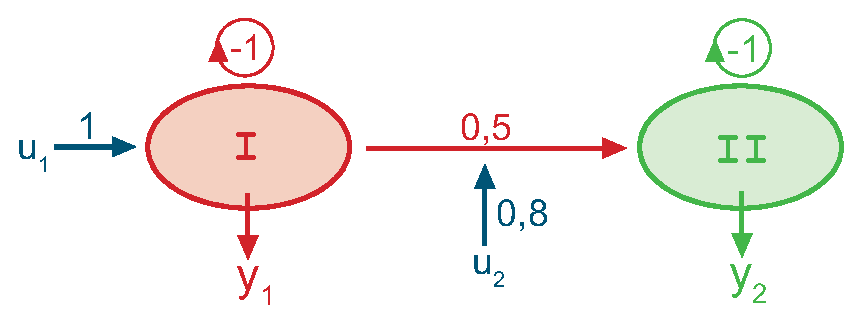
\includegraphics[width=0.8\linewidth]{res/bilinearesModel_bunt_lin_werte.eps}}
		\end{figure}
		\centering{\colorbox{maincolor!10}{
		$
		\dot{z}(t)=A\cdot z(t)+\sum_{j}u_jB^j\cdot z(t)+C\cdot u(t)
		$}}
		\begin{align*}
		& A  =
		\begin{pmatrix}
		-1 & 0 \\ 0.5 & -1 
		\end{pmatrix} &
		& B_1 = 0  
		 & B_2 =
		\begin{pmatrix}
		0 & 0 \\ 0.8 &  0
		\end{pmatrix} & 
		 & C =
		\begin{pmatrix}
		1 & 0 \\  0 &  0
		\end{pmatrix} 
		\end{align*}
	\end{frame}
	\begin{frame}[t]{Simulation eines 2-Regionen-Systems}
		\centering
		\begin{figure}
			\vspace*{-0.53cm}
			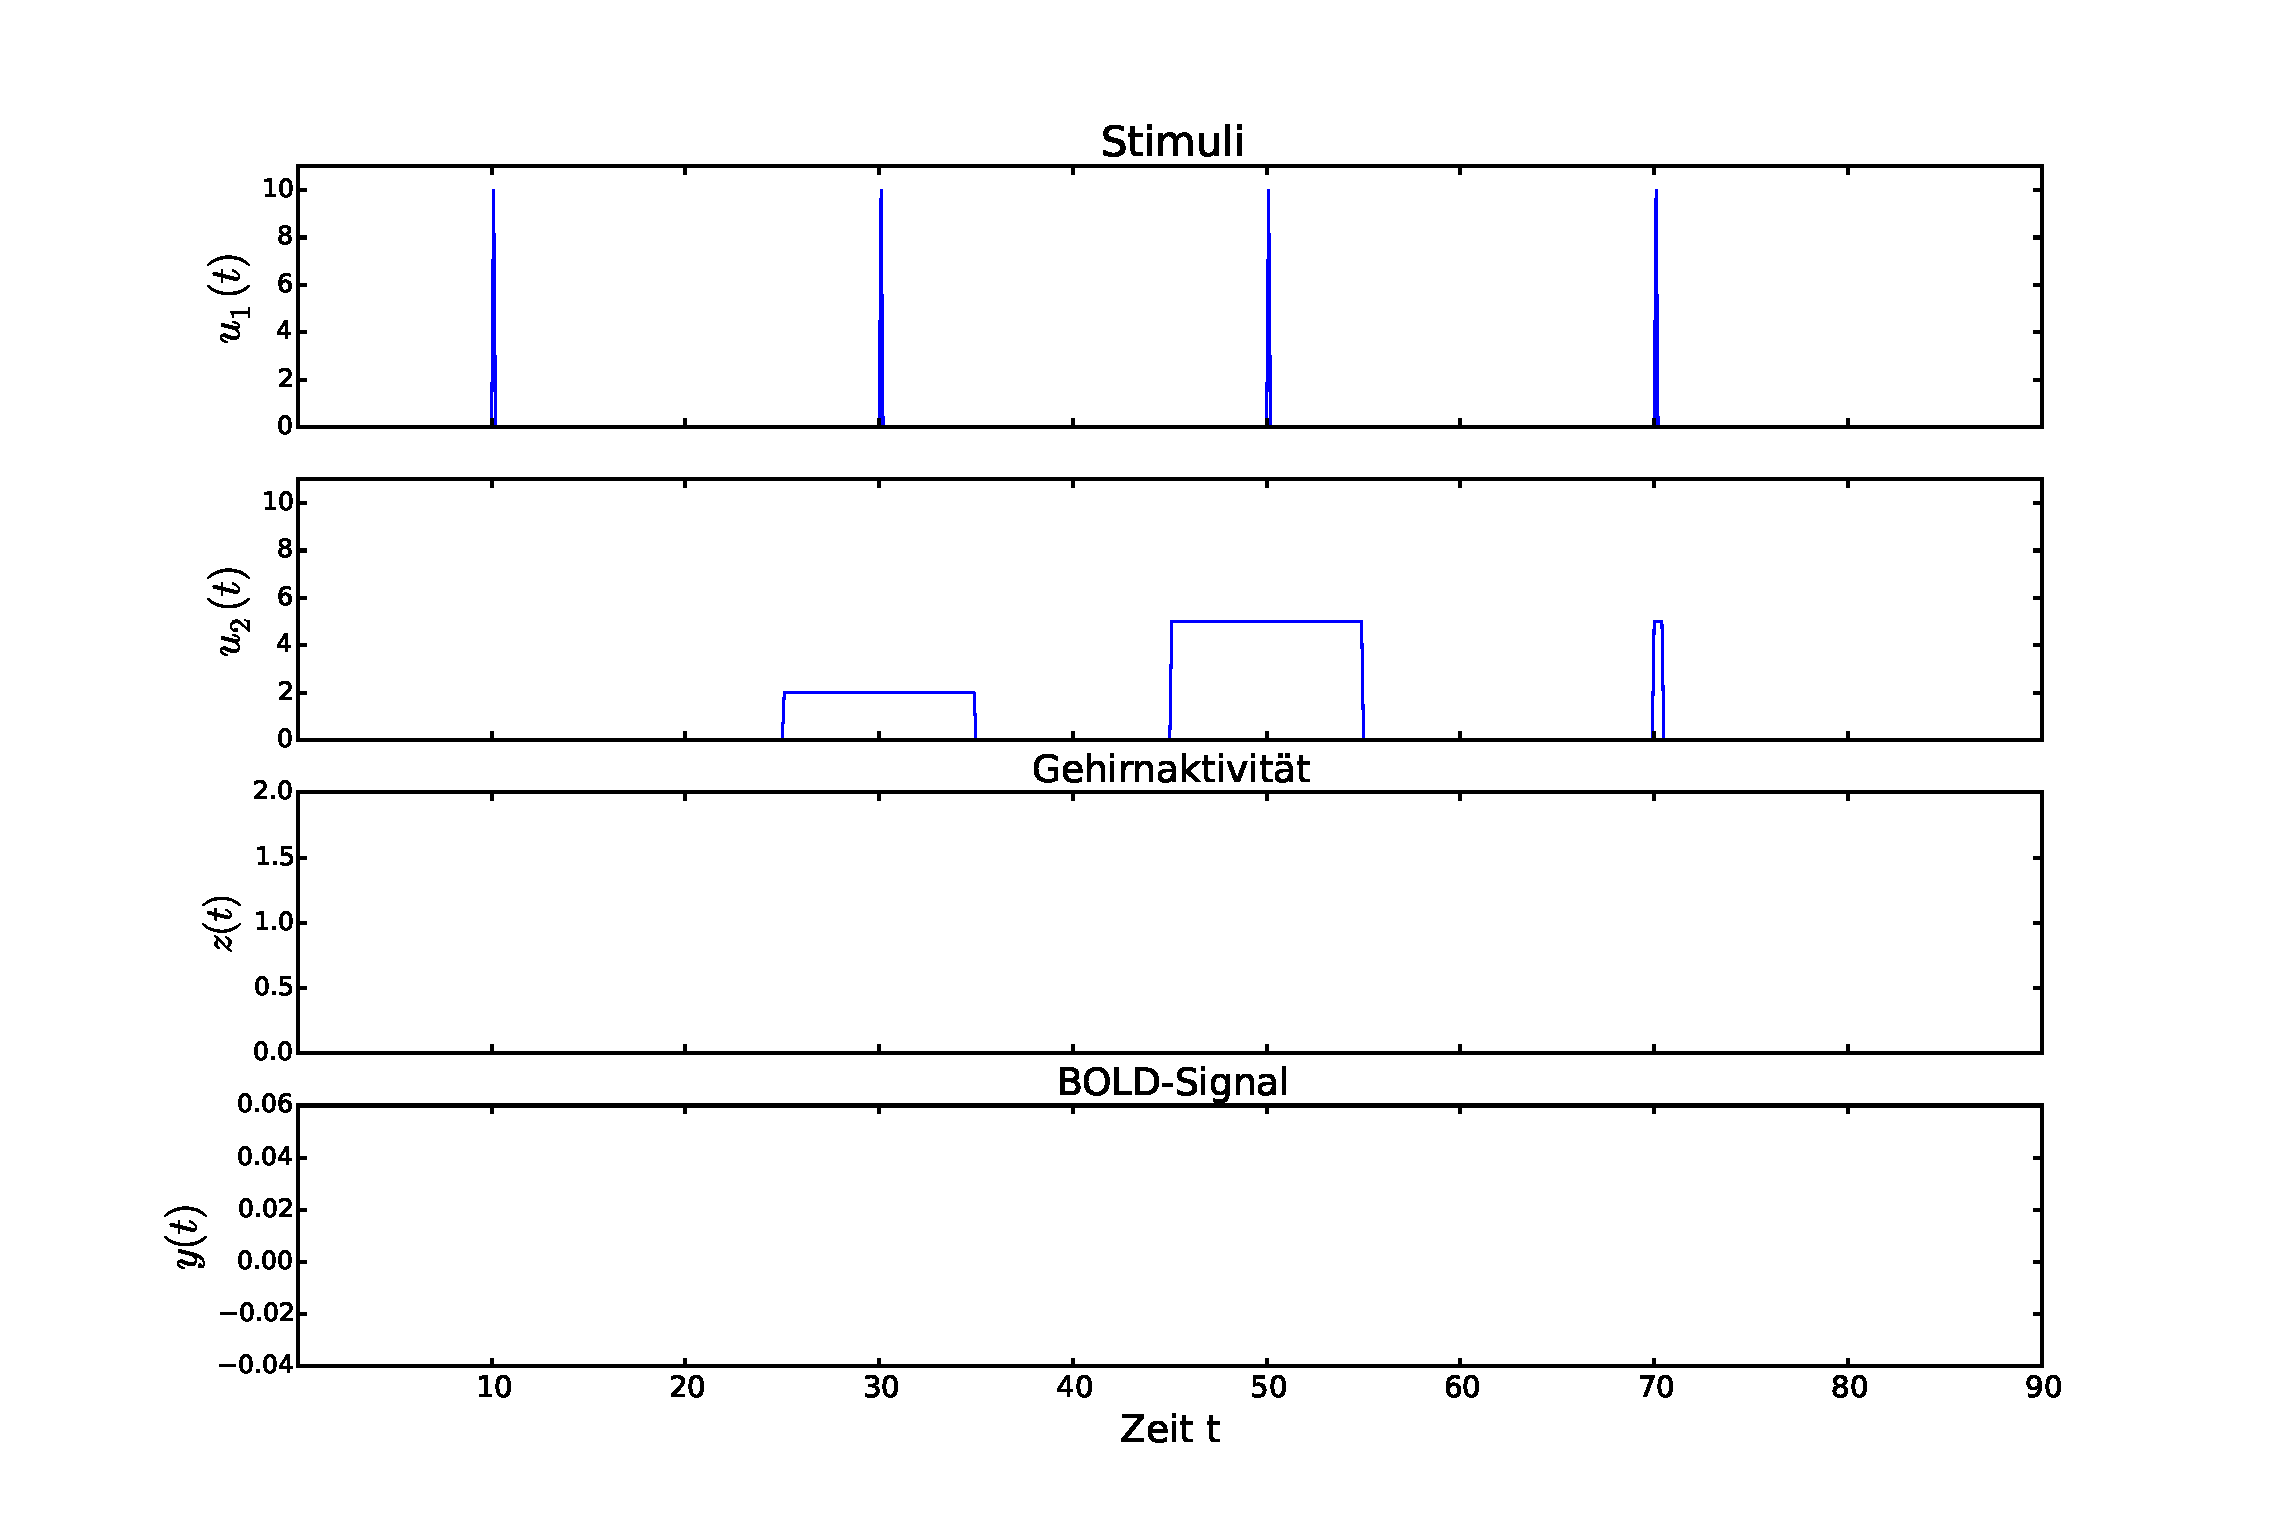
\includegraphics[width=0.975\linewidth ]{res/hemodynamicExample-2-stimulus.eps}
		\end{figure}
		\begin{tikzpicture}[remember picture,overlay]
			\node[at=(current page.center), xshift=4cm, yshift=3.5cm]{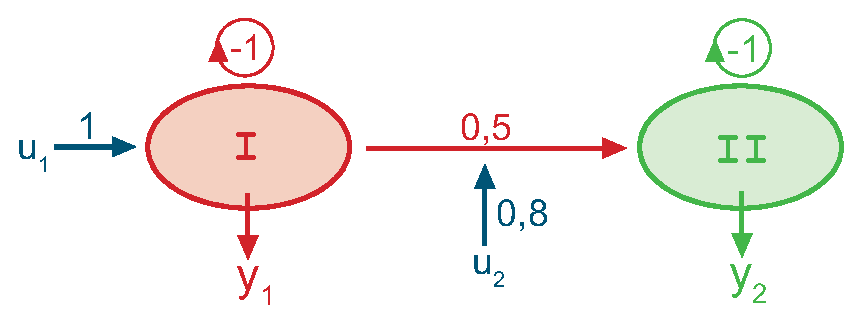
\includegraphics[width=0.35\linewidth ]
				{res/bilinearesModel_bunt_lin_werte.eps}};
		\end{tikzpicture}
		\vskip0pt plus 1filll
	\end{frame}
	\begin{frame}[t]{Simulation eines 2-Regionen-Systems}
		\begin{figure}
			\vspace*{-0.53cm}
			{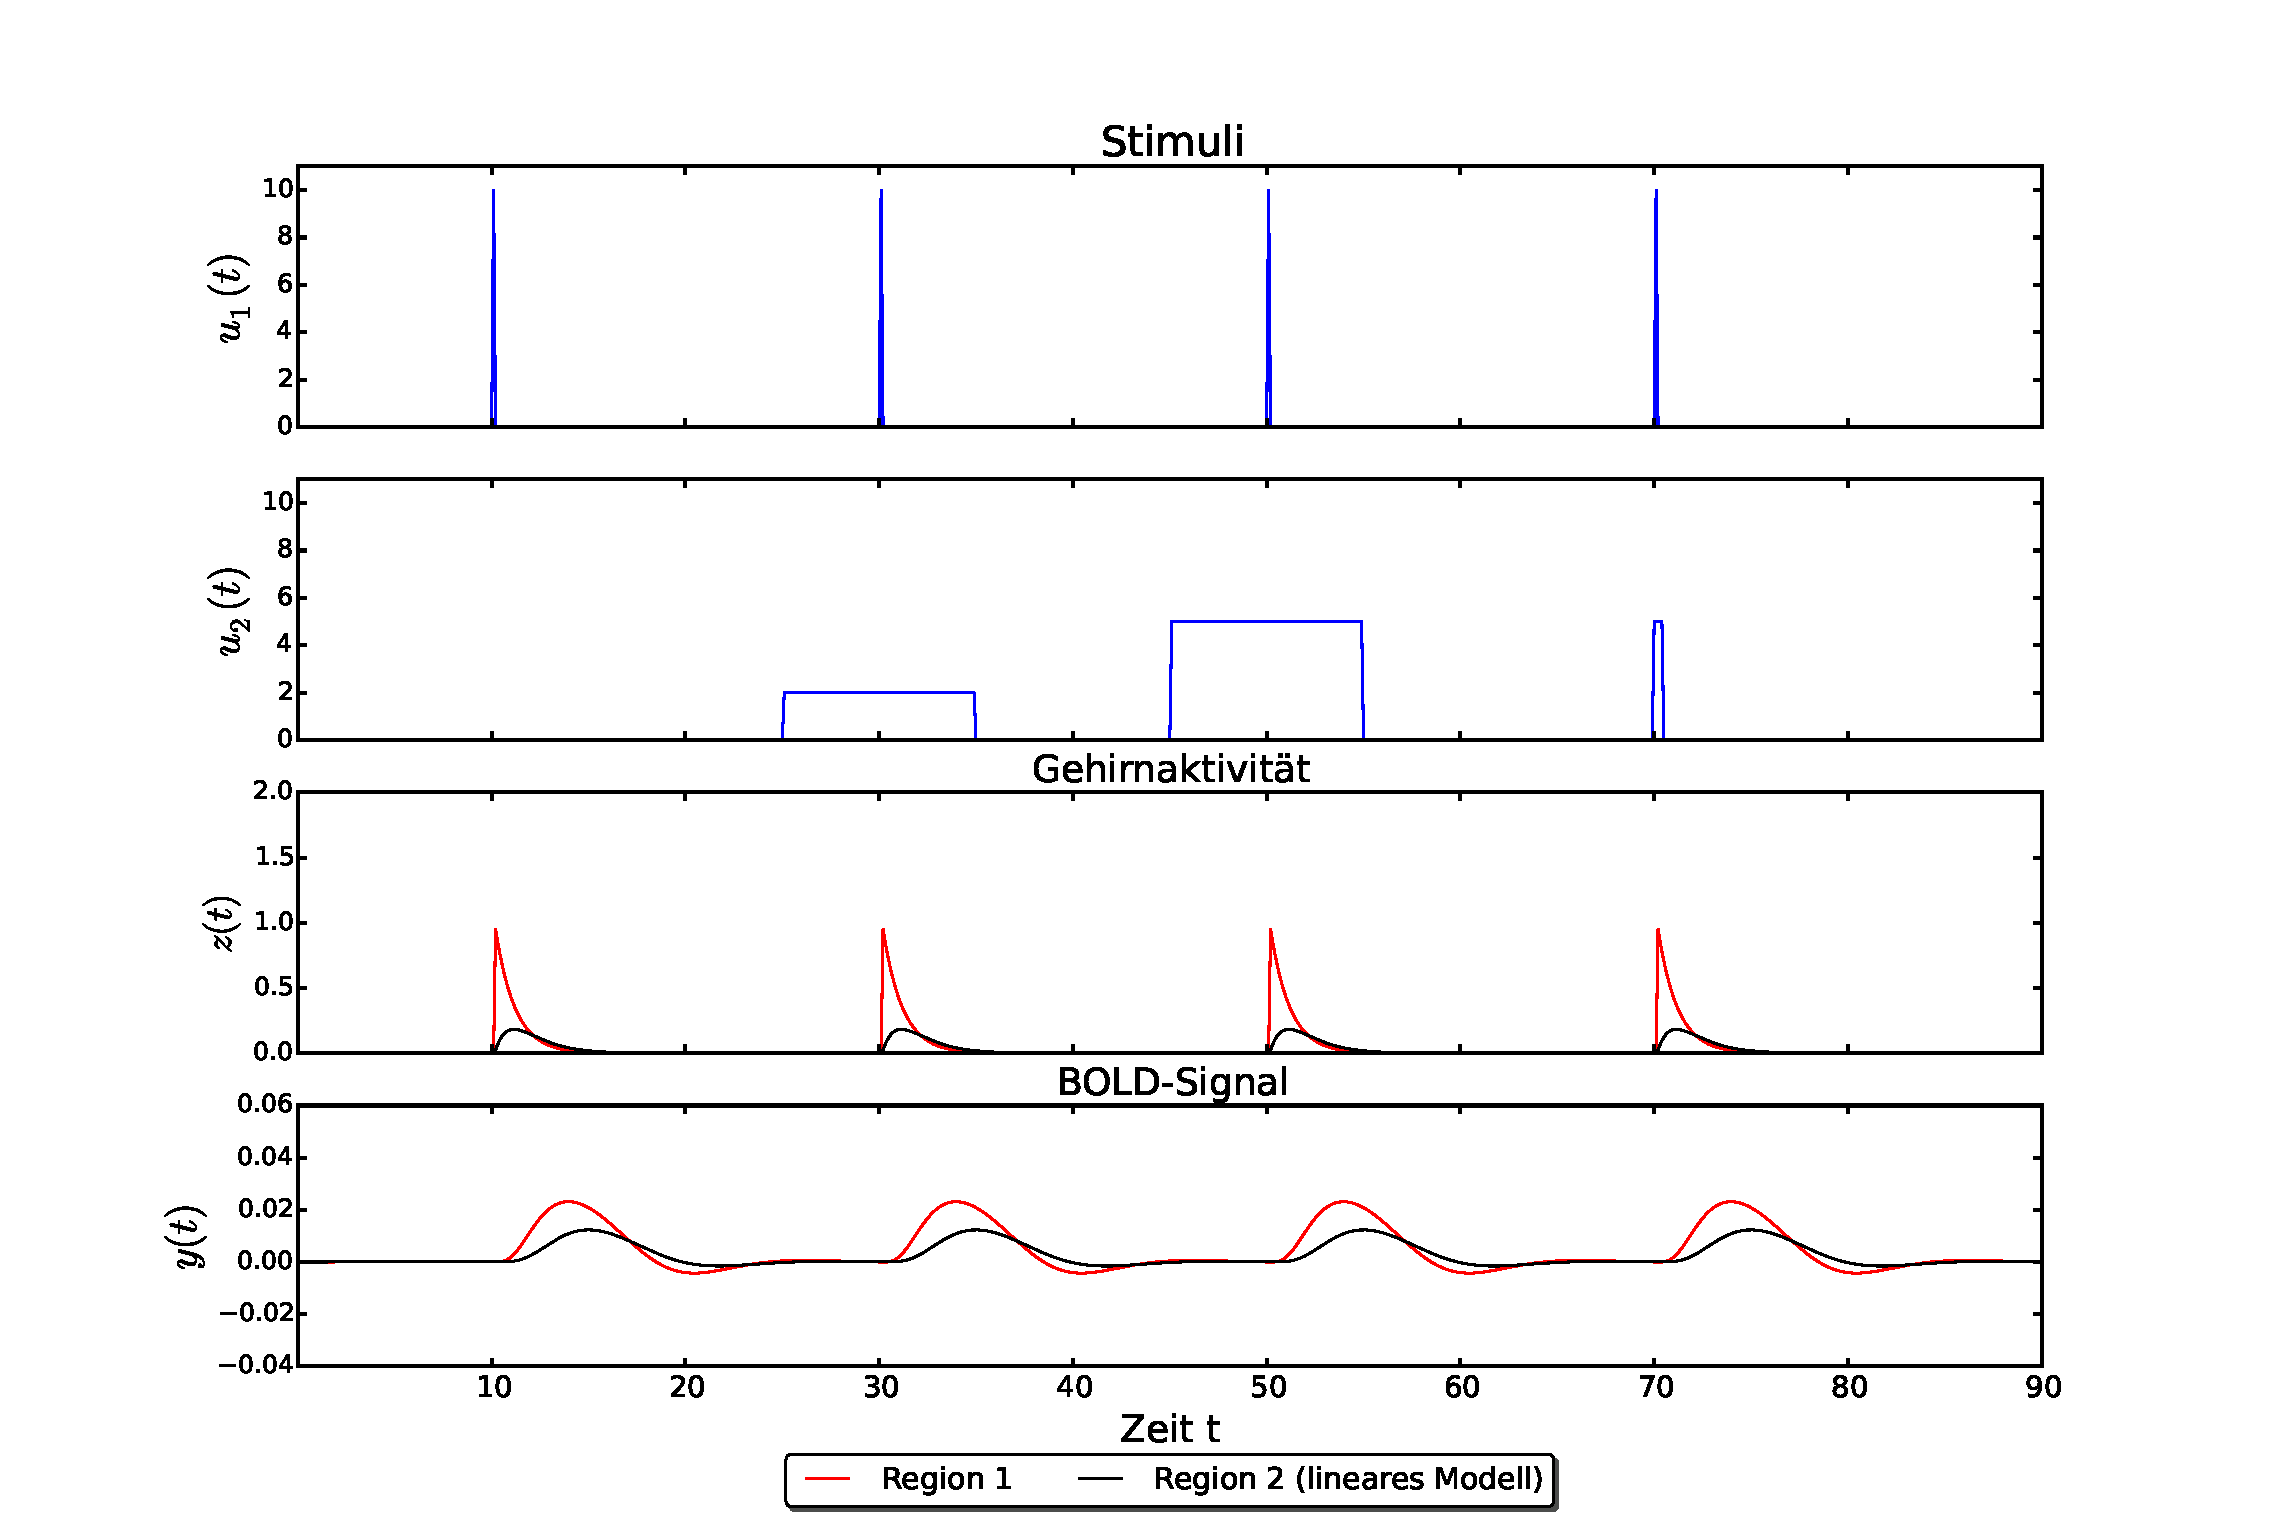
\includegraphics[width=0.975\linewidth]{res/hemodynamicExample-2-linear.eps}}
		\end{figure}
		\begin{tikzpicture}[remember picture,overlay]
			\node[at=(current page.center), xshift=4cm, yshift=3.5cm] {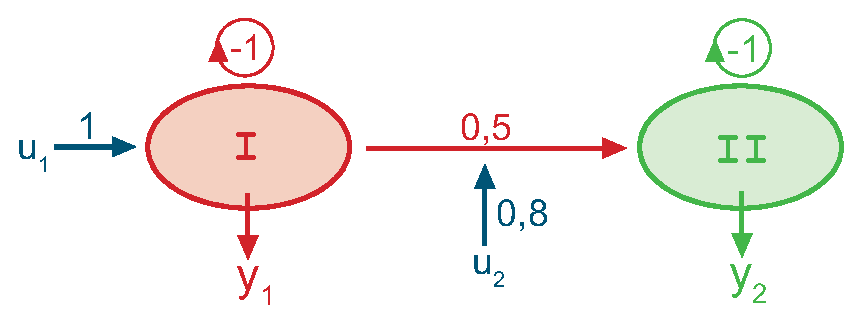
\includegraphics[width=0.35\linewidth ]
				{res/bilinearesModel_bunt_lin_werte.eps}};
		\end{tikzpicture}
		%\vskip0pt plus 1filll
	\end{frame}
	\begin{frame}[t]{Simulation eines 2-Regionen-Systems}
		\begin{figure}
			\vspace*{-0.53cm}
			{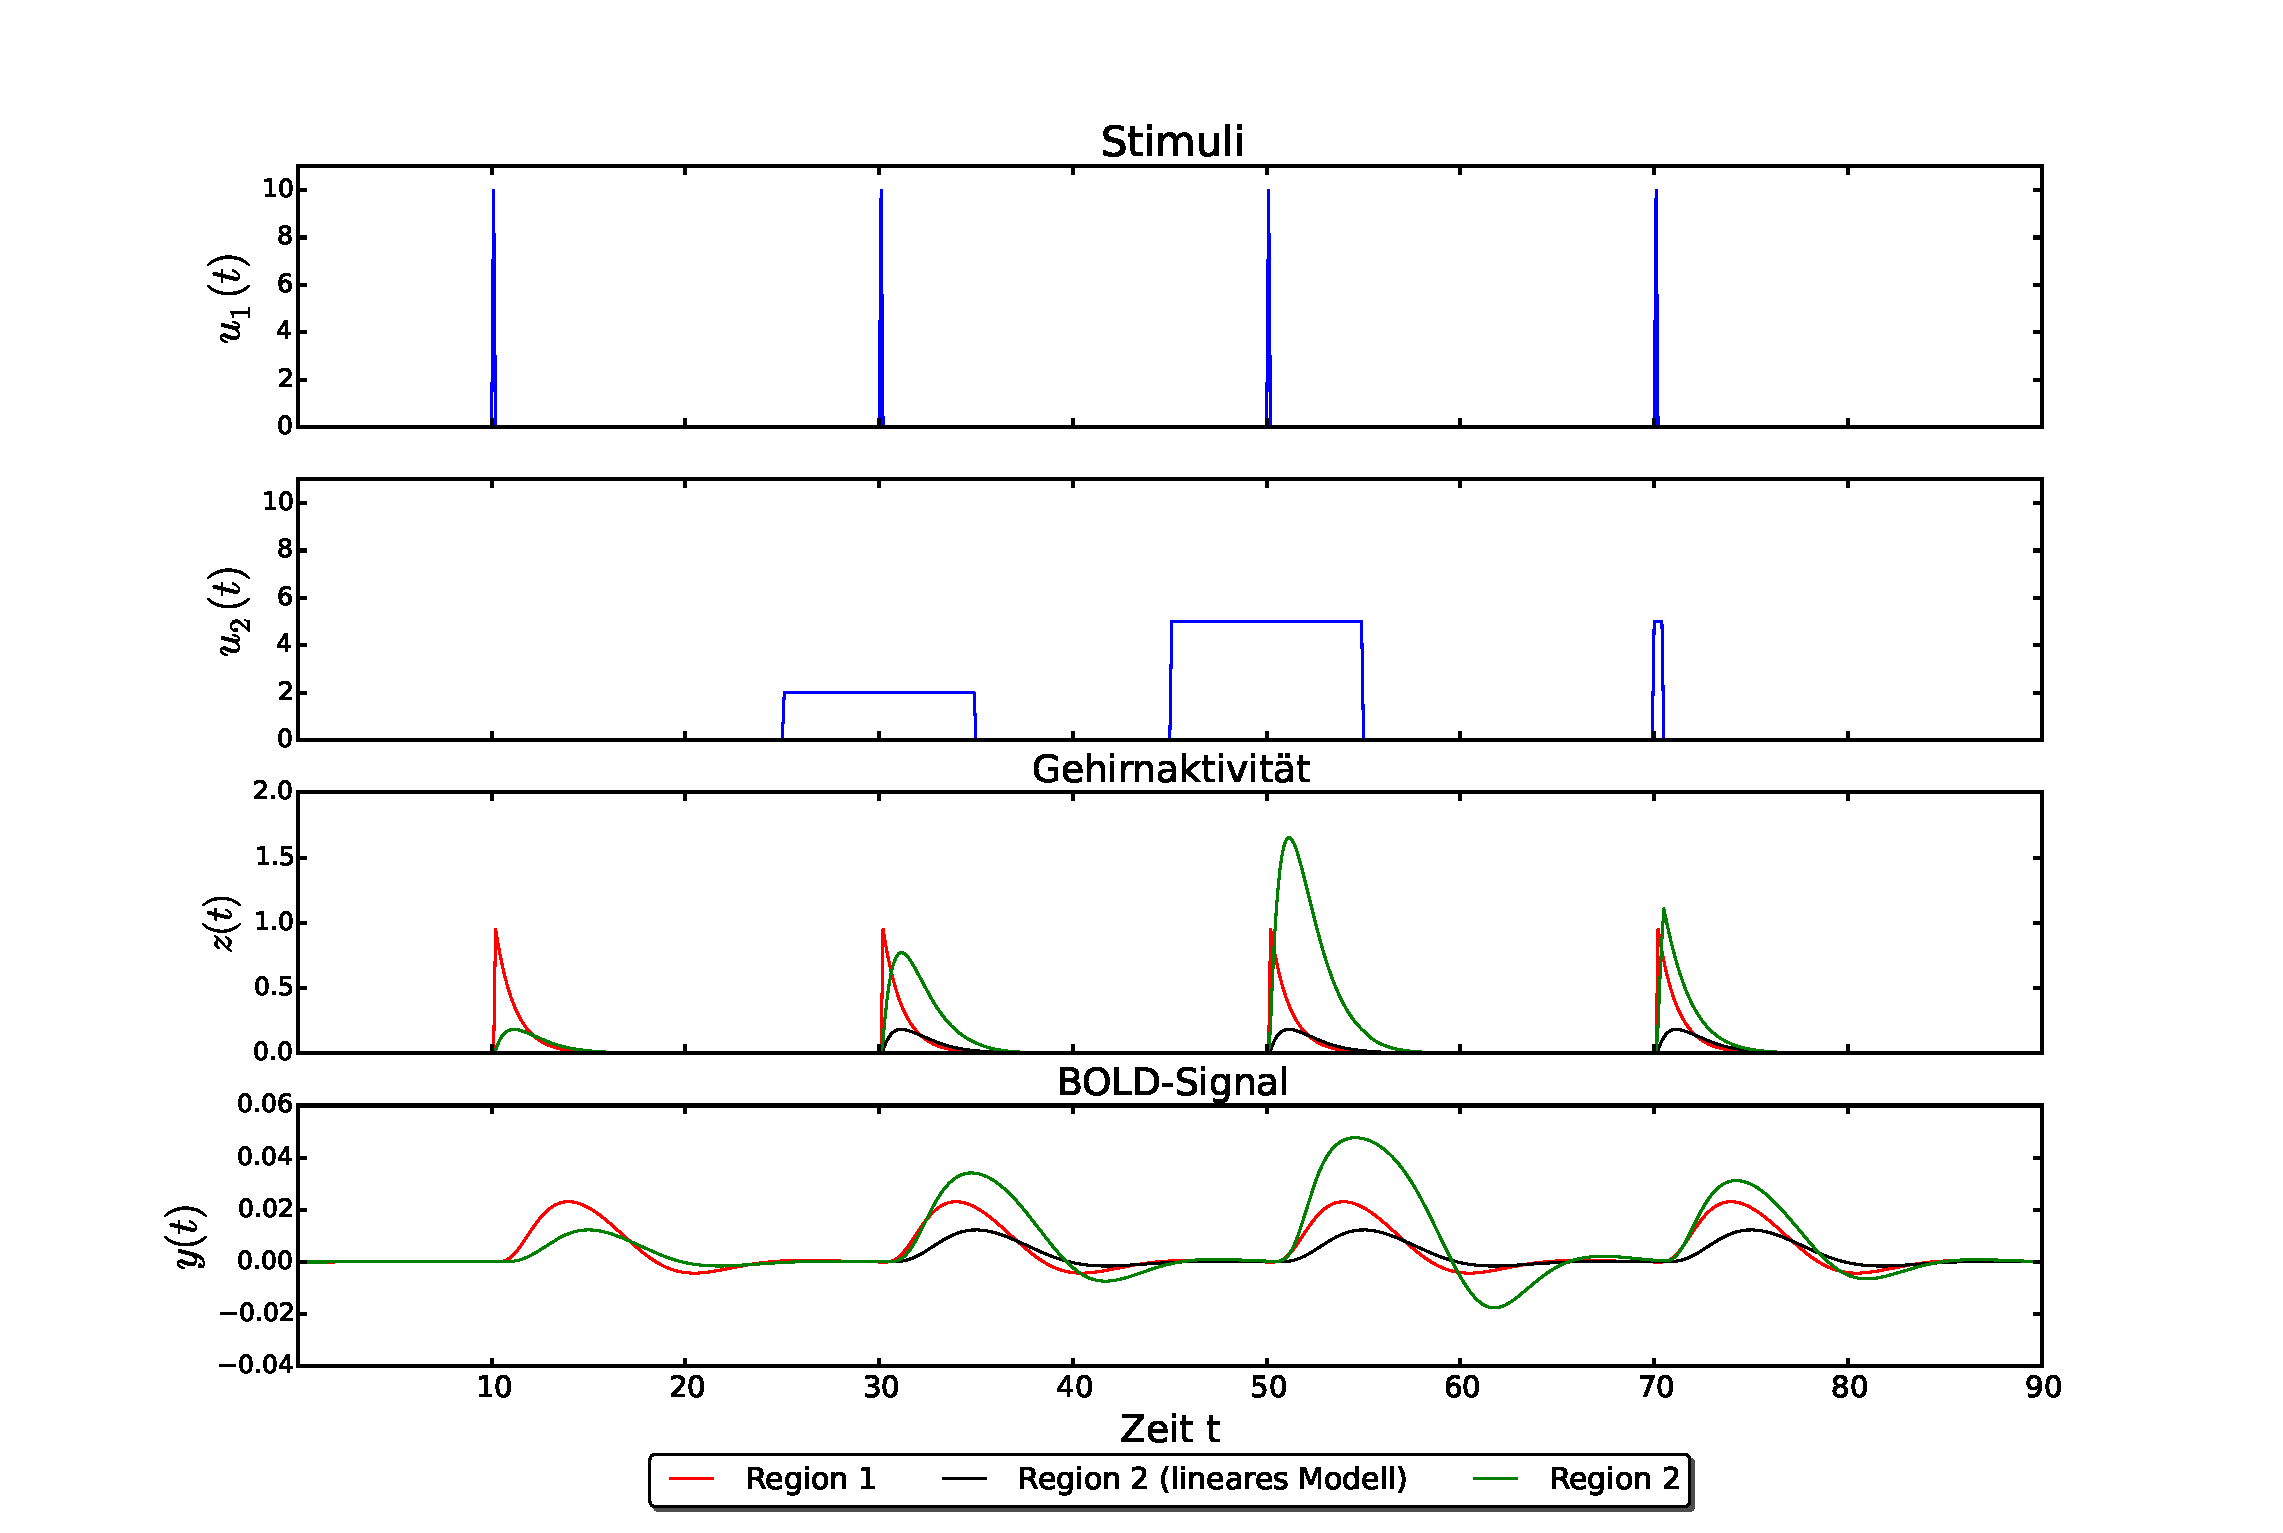
\includegraphics[width=0.975\linewidth ]{res/hemodynamicExample-2-bilinear.eps}}
		\end{figure}
		\begin{tikzpicture}[remember picture,overlay]
			\node[at=(current page.center), xshift=4cm, yshift=3.5cm]{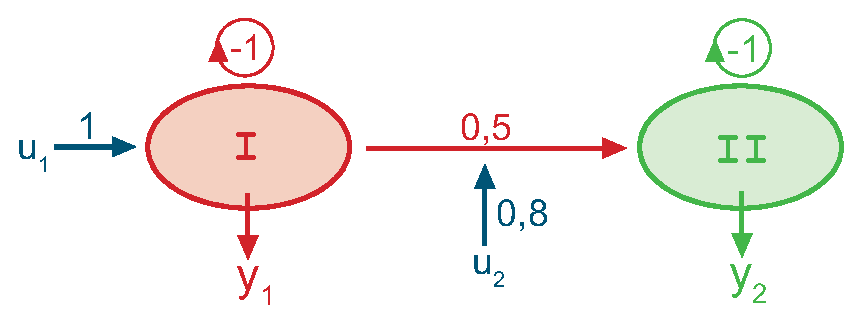
\includegraphics[width=0.35\linewidth ]
				{res/bilinearesModel_bunt_lin_werte.eps}};
		\end{tikzpicture}
		%\vskip0pt plus 1filll
	\end{frame}

\begin{frame}[t]{Zusammenfassung und Ausblick}
	\begin{columns}
		\column[t]{6.8cm}
		\vspace{-0.5 cm}
		\begin{itemize}
			\item \textit{Ziel:} \\Modellierung von Interaktionen in einem neuronalen Netzwerk\\[0.5cm]
			\item \textit{Ansatz:} \\Taylorentwicklung bis zur 2ten Ordnung für die neuronale Aktivität \\[0.5cm]
			\item \textit{Vergleichbarkeit mit Experiment:} \\ Hämodynamisches Modell Variation des Blutvolumens und des desoxygenierten Hämoglobins
		\end{itemize}
		\column[t]{6cm}
		\begin{figure}
			\centering
			\vspace{-1cm}
			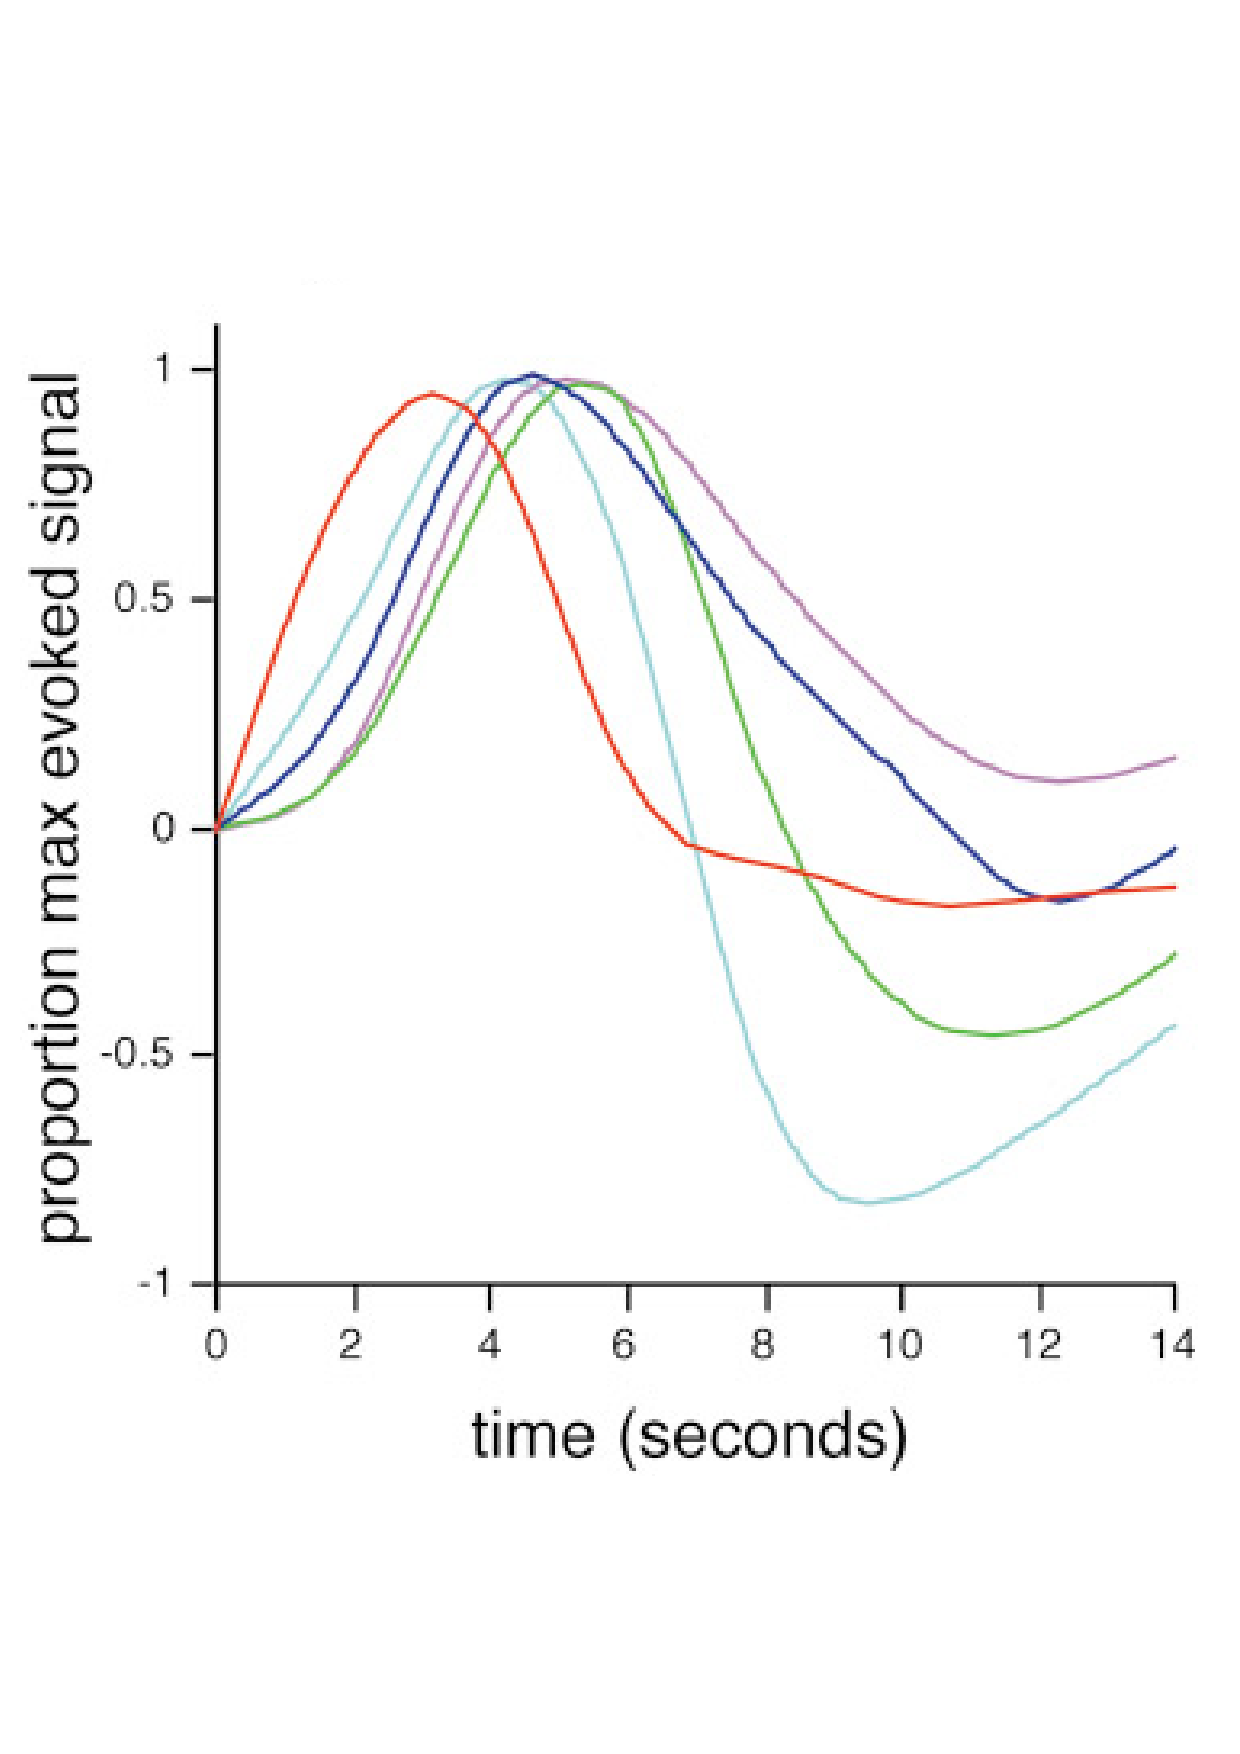
\includegraphics[width=0.98\linewidth]{res/Aguirre1998-BOLD-hemodynamic-responses.pdf}
			\vspace{-0.1cm}
			\caption*{\scriptsize Hämodynamische Antworten einer Gruppe von fünf Probanden. \\ (nach Aguirre et al., NeuroImage \textbf{8}, 1998)}
		\end{figure}
	\end{columns}
\end{frame}

%%%%%%%%%%%%%%%%%%%%%%%%%%%%%%% Ende
\begin{frame}
\centering
\huge Danke für die Aufmerksamkeit!
\end{frame}


\section{Literatur}
	\begin{frame}{Literatur}
		\begin{itemize}
			\item \textit{Dynamic causal modelling} \\ {\small K.J. Friston et al. / NeuroImage 0 (2003)} \\ {\footnotesize \url{web.mit.edu/swg/ImagingPubs/connectivity/Dcm_Friston.pdf}}
%			\item \textit{{\small Bayesian Estimation of Dynamical Systems: An Application to fMRI}} \\ {\small K.J. Friston / NeuroImage (2002)} \\ {\footnotesize \url{www.sciencedirect.com/science/article/pii/S1053811901910444}}
		\end{itemize}
	\end{frame}

%%%%%%%%%%%%%%%%%%%%%%%%%%%%%%%%% Backupfolien
\begin{frame}[t]{Simulation eines 2-Regionen-Systems}
		\begin{figure}
			\vspace*{-0.53cm}
			{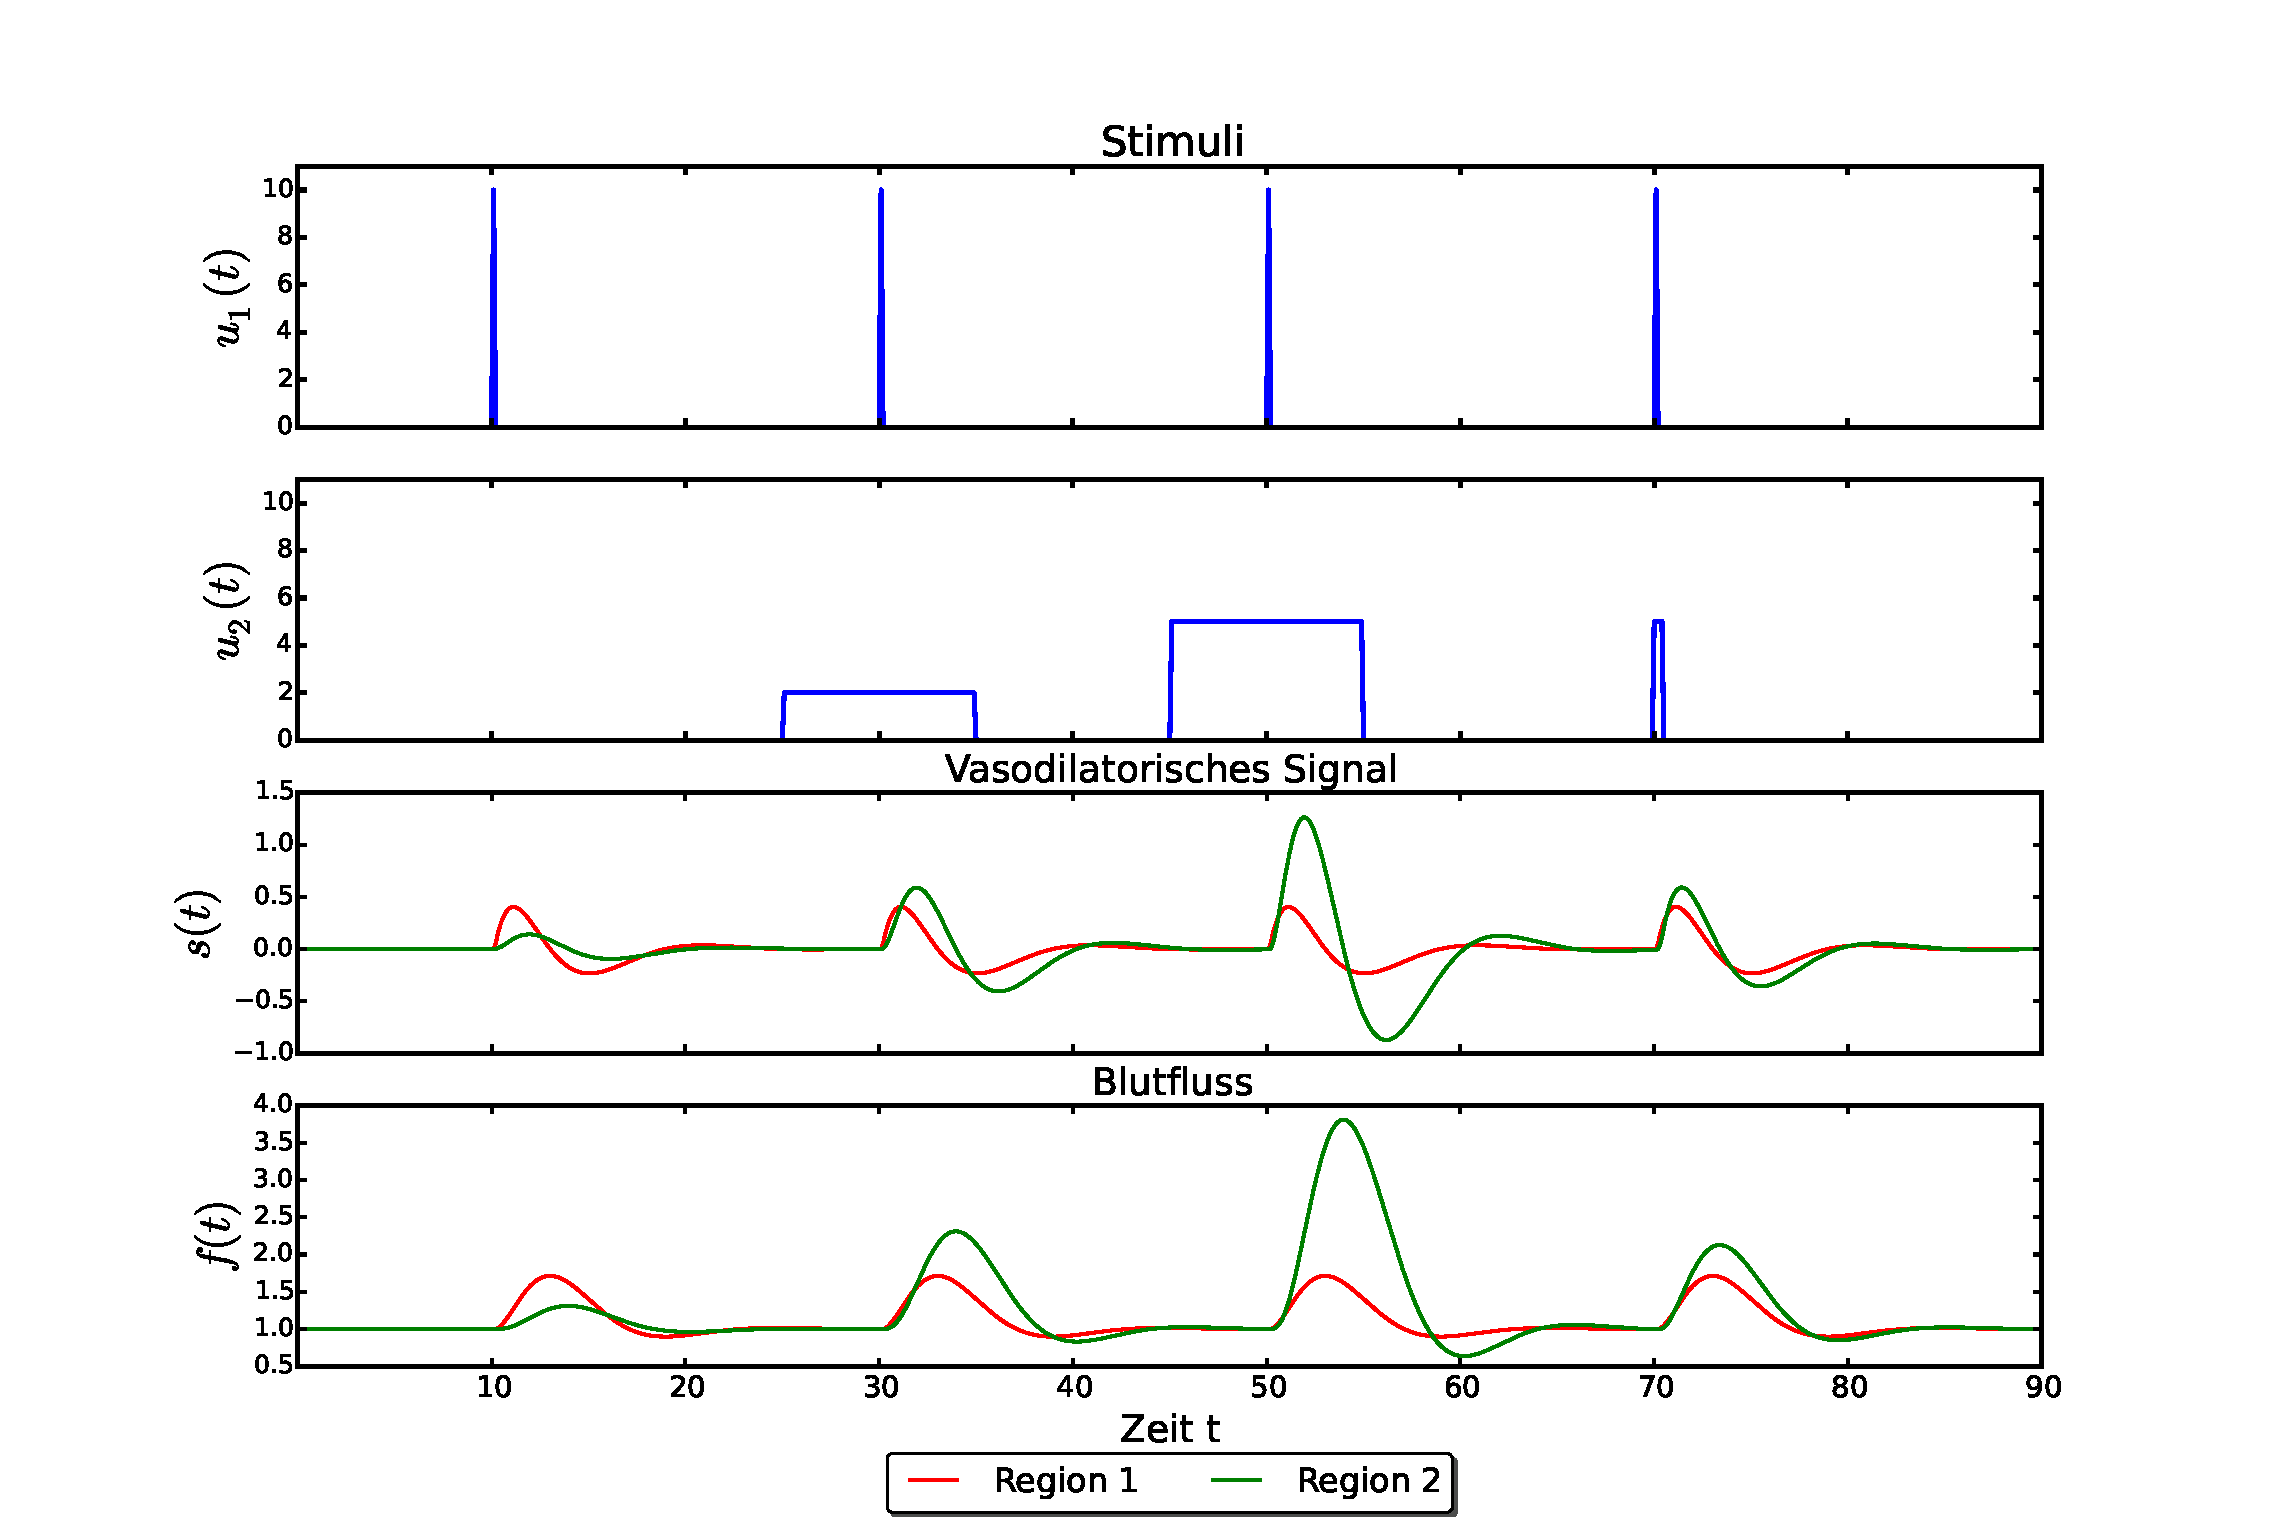
\includegraphics[width=0.975\linewidth ]{res/hemodynamicExample-2-signal-fluss.eps}}
		\end{figure}
		\begin{tikzpicture}[remember picture,overlay]
			\node[at=(current page.center), xshift=4cm, yshift=3.5cm]{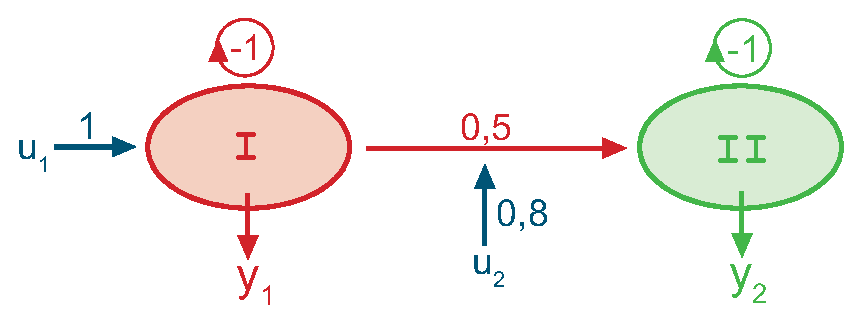
\includegraphics[width=0.35\linewidth ]
				{res/bilinearesModel_bunt_lin_werte.eps}};
		\end{tikzpicture}
		%\vskip0pt plus 1filll
\end{frame}
\begin{frame}[t]{Simulation eines 2-Regionen-Systems}
		\begin{figure}
			\vspace*{-0.53cm}
			{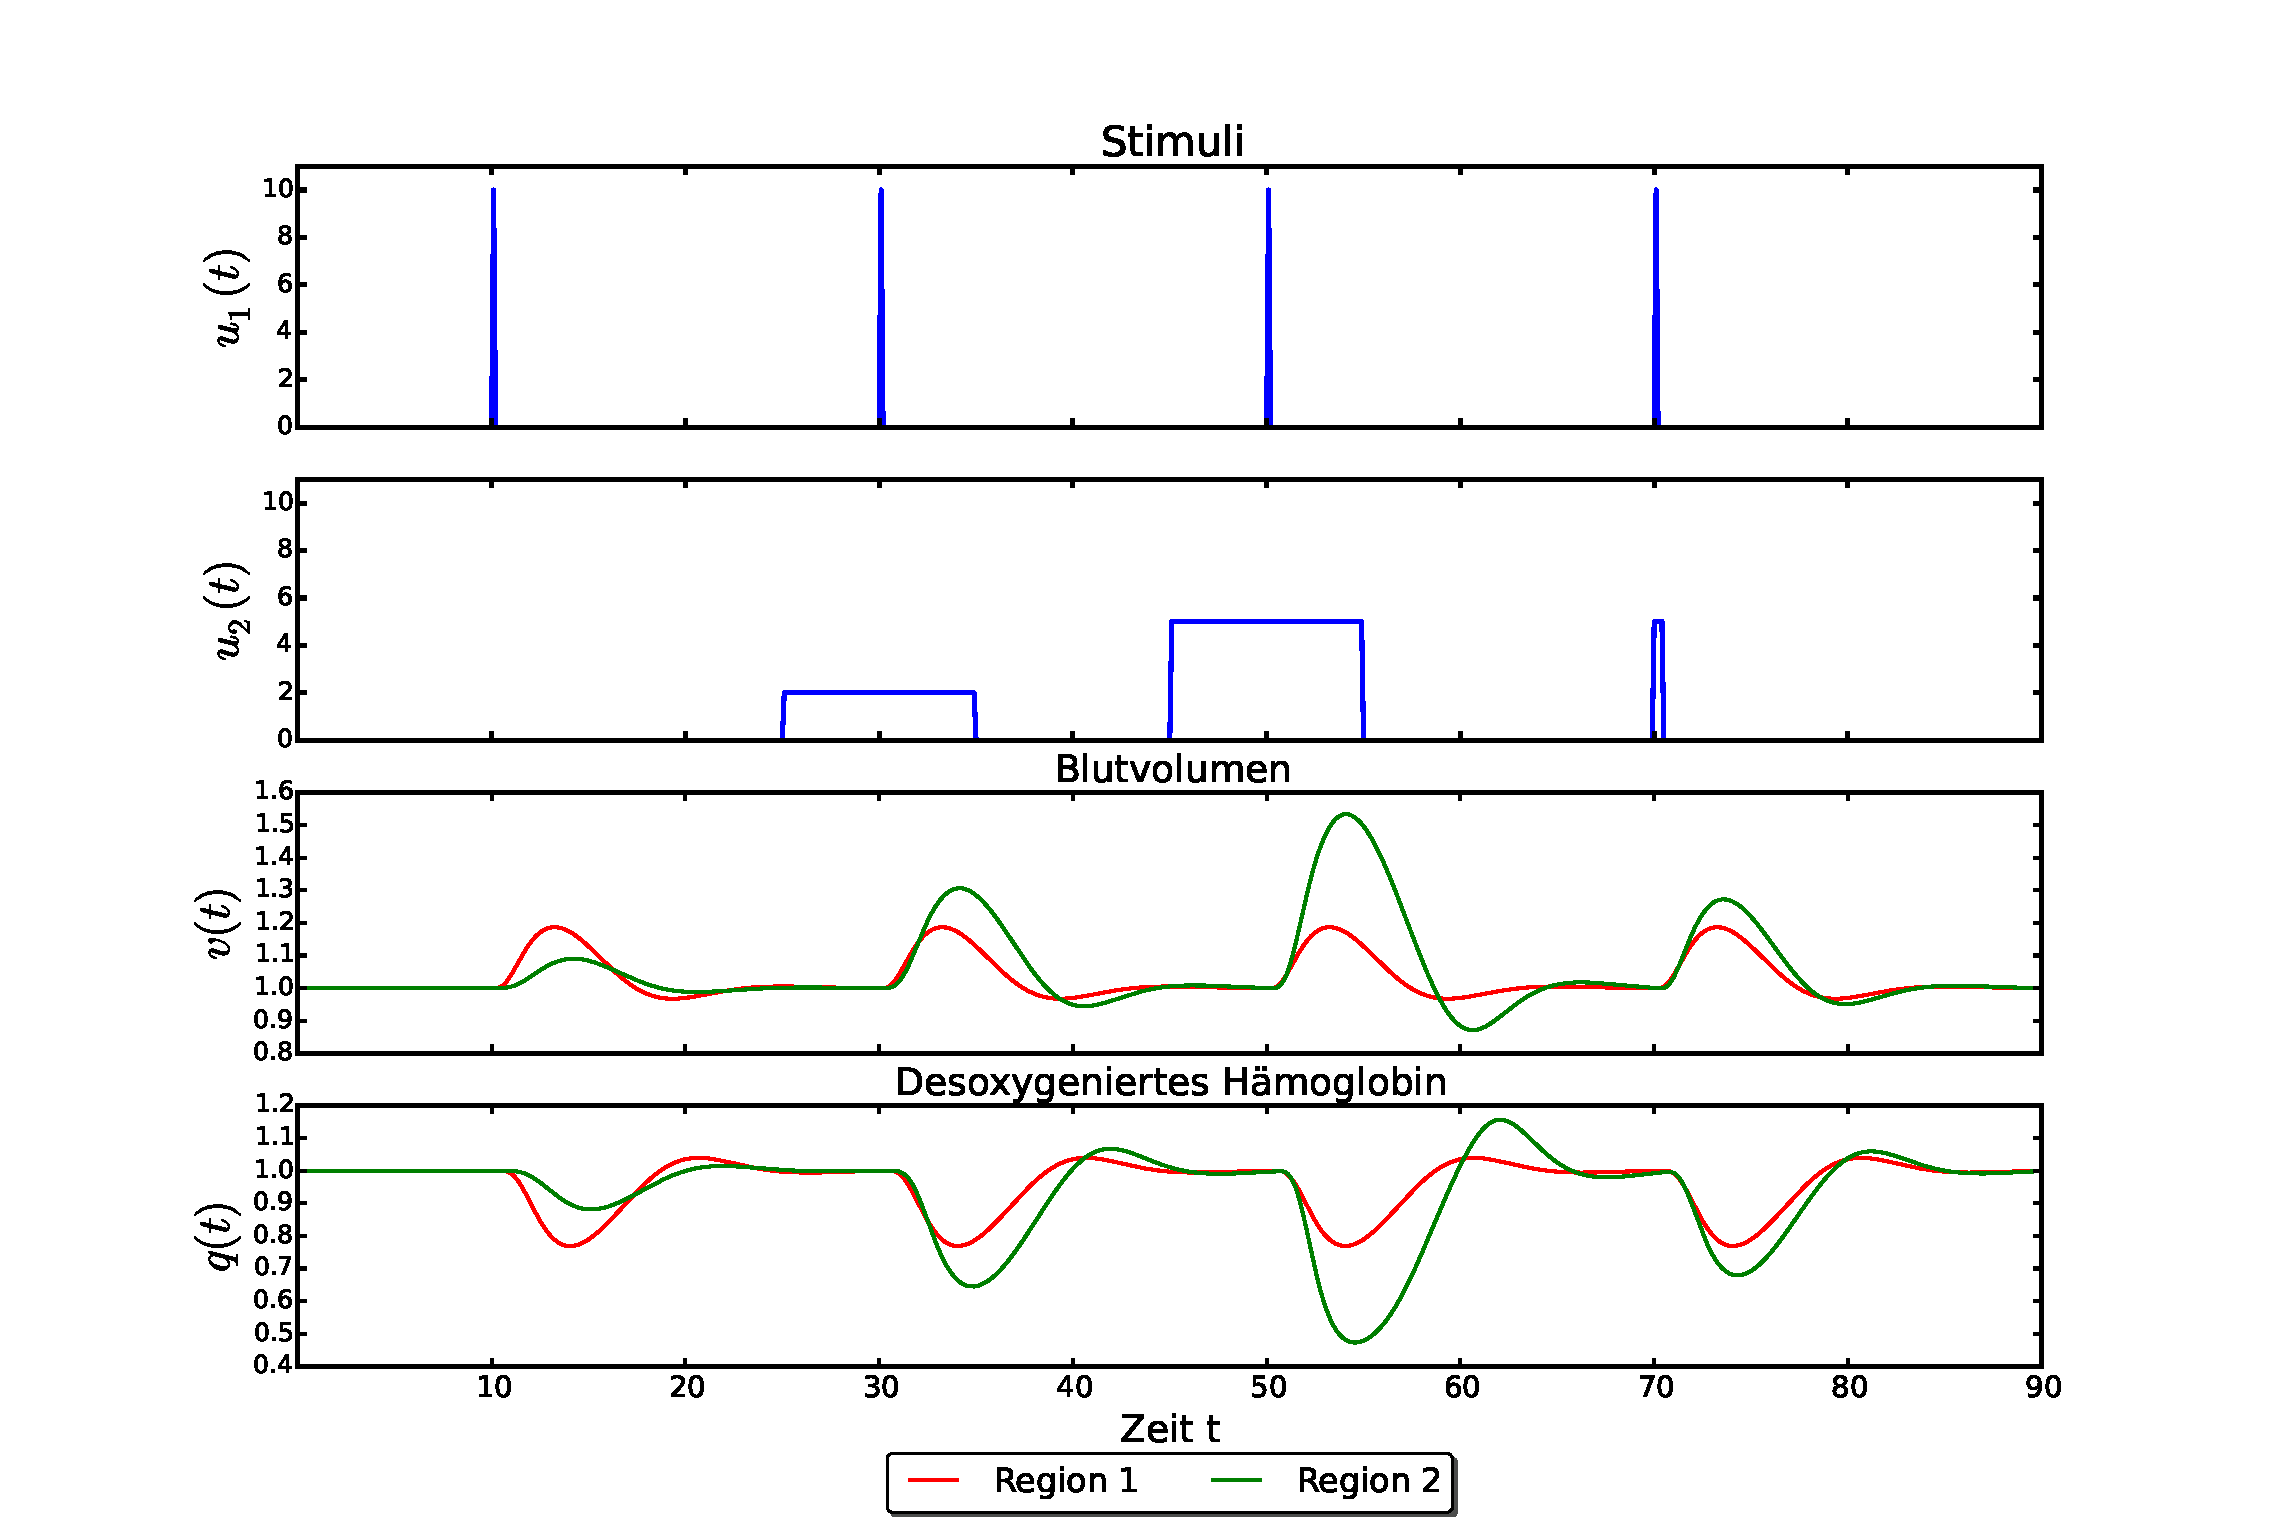
\includegraphics[width=0.975\linewidth ]{res/hemodynamicExample-2-volumen-deshb.eps}}
		\end{figure}
		\begin{tikzpicture}[remember picture,overlay]
			\node[at=(current page.center), xshift=4cm, yshift=3.5cm]{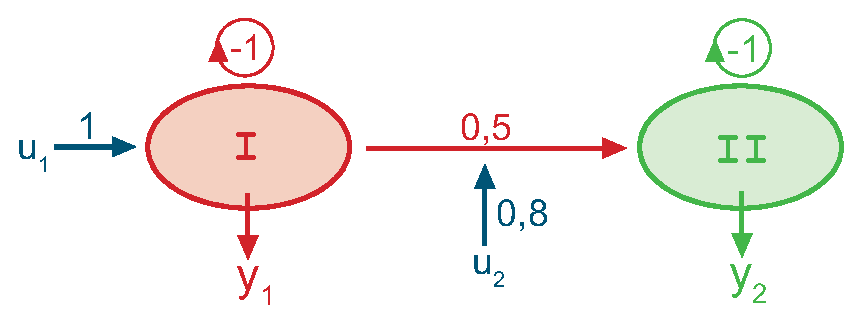
\includegraphics[width=0.35\linewidth ]
				{res/bilinearesModel_bunt_lin_werte.eps}};
		\end{tikzpicture}
		%\vskip0pt plus 1filll
\end{frame}


%\begin{frame}
%	\frametitle{Designfeatures}
%	\begin{block}{Hervorhebungen}
%	 \textbf{Wenn man Dinge hervorheben möchte nutzt man entweder Fettdruck,} \textit{ kursive Schrift} \alert{ oder das Schlüsselwort "alert"}. Auch "itemize"-Umgebungen werden von der Stilvorlage überschrieben:
%	\end{block}
%	\pause
%	\begin{itemize}
%	 \item So wird sichergestellt,
%	 \item dass alle Elemente der Präsentation 
%	 \item dieselbe Farbe nutzen.
%	\end{itemize}
%	\begin{alertblock}{Achtung!}
%	 Hier kommt Rot ins Spiel!	
%	\end{alertblock}
%	\begin{exampleblock}{Beispiel}
%	 Hier kommt Grün ins Spiel!
%	\end{exampleblock}
%\end{frame}

\end{document}
